
\documentclass[rascunho]{fei}
\usepackage[utf8]{inputenc}
%\usepackage[brazilian]{babel}
\usepackage{verbatim}

\usepackage[caption=false]{subfig}
\usepackage{float}
\usepackage{amssymb}

%\usepackage{subfigure}
%\selectlanguage{brazilian}

\author{Claudio de Oliveira Vilão Junior}
\title{UM SISTEMA DE VISÃO COMPUTACIONAL MONOCULAR PARA UM ROBÔ MÓVEL HUMANOIDE}
%\subtitulo{CONTROLE SERVO-VISUAL DE JOGADORES DE FUTEBOL DE ROBÔS humanoides}
%\cidade{Cidade}
%\instituicao{Instituição de Ensino}

\begin{document}
\overfullrule=2cm
\maketitle

\begin{folhaderosto}
Dissertação de Mestrado apresentada ao Centro Universitário da FEI para obtenção do título de Mestre em Engenharia Elétrica, orientado pelo Prof. Dr. Reinaldo Augusto da Costa Bianchi.
\end{folhaderosto}

\fichacatalografica
\folhadeaprovacao
\dedicatoria{A meus pais.}

\begin{agradecimentos}
Agradeço pelo incentivo que me foi dado em momentos de dificuldade por todos os meus familiares, em especial meus pais Anna Maria Cortezi Oliveira Vilão e Claudio de Oliveira Vilão. 

Preciso agradecer, com uma ênfase maior, o Prof. Dr. Reinaldo Augusto da Costa Bianchi por me ajudar e suportar em todos os momentos que passei durante este período, mas principalmente por acreditar no meu trabalho e em mim. Não posso deixar de mencionar, e talvez nem precise,  mas, gostaria de agradecer pelas oportunidades que tem me dado, além do apoio, da motivação, das críticas construtivas e das aulas. Muito obrigado Professor.

Aos professores do Centro Universitário da FEI pelo incentivos e pelas aulas ministradas: Prof. Dr. Carlos Eduardo Thomaz, Prof. Dr. Flávio Tonidandel, Prof. Dr. Paulo Sérgio Silva Rodrigues, Prof. Dr. Paulo E. Santos.

Agradeço ao colega Ms. Isaac Jesus da Silva por sua contribuição me ajudando nas pesquisas científicas que vem sendo desenvolvidas com sugestões e críticas construtivas.
Agradeço aos colegas Ms. Danilo Hernani Perico e Ms. Thiago Pedro Donadon Homem por terem me ajudado com sugestões e críticas, mas também transmitindo motivação e foco.

Agradeço à minha esposa Mônica Farias da Silva pelo suporte e paciência, além de auxílio e dicas do tratamento de imagens.

Agradeço a Deus.
\end{agradecimentos}

\epigrafe{A good scientist is a person with original ideas.}{Freeman Dyson}

\begin{resumo}

\begin{comment}
Uma única imagem representa um conjunto de dados de tamanho considerável e tipicamente várias operações precisam ser feitas em cada pixel da referida imagem. Em uma estrutura de vídeo, a qual pode ser assimilado como uma sucessão de várias imagens, esta tarefa torna-se ainda mais difícil, já que, a taxa de quadros por segundo necessita ser mantida mesmo com a câmera em movimento. Este trabalho pretende descrever um sistema de visão monocular para quatro robôs humanoides desenvolvidos para participar da liga humanoide na categoria Kid Size, da RoboCup. O sistema de visão proposto permite que os robôs sejam capazes de acompanhar uma bola e detectar companheiros e adversários, fornecendo informações, tais como, distâncias e orientações de todos esses objetos simultaneamente, de forma que, todos os processos possam ser executados em tempo real com diferentes resoluções de câmera. Devido a mudança constante de regras da competição, aumentando cada vez mais a complexidade do ambiente, o uso de técnicas de alto nível, ainda pouco começam a parecer atraentes. Dessa forma o uso do Haar-Adaboost e do HOG-SVM para detecção de objetos pertencentes ao jogo, apresentaram resultados relevantes. Técnicas de baixo, médio e alto nível foram utilizadas em nossos robôs com poucas adversidades, com taxa de quadros por segundo condizentes com um robô de ação rápida e com a capacidade de generalização e identificação dos objetos demonstrados nas Curvas de Características de Operação do Receptor (ROC). 
\end{comment}

Uma única imagem representa um conjunto de dados de tamanho considerável e tipicamente várias operações precisam ser feitas em cada pixel da referida imagem. Em uma estrutura de vídeo, a qual pode ser descrita como uma sucessão de várias imagens, esta tarefa torna-se ainda mais difícil, já que a taxa de quadros analisadas necessita ser mantida mesmo com a câmera em movimento. Este trabalho descreve um sistema de visão monocular para quatro robôs humanoides desenvolvidos para participar da liga humanoide na categoria KidSize, da RoboCup. O sistema de visão proposto permite que os robôs acompanhem uma bola e detectem companheiros e adversários, fornecendo informações  como  distâncias e orientações de todos esses objetos simultaneamente, de forma que, todos os processos possam ser executados em tempo real com diferentes resoluções de câmera. Devido a mudança constante de regras da competição, aumentando cada vez mais a complexidade do ambiente, o uso de técnicas de alto nível começam a parecer atraentes. Dessa forma o uso do Haar-Adaboost e do HOG-SVM para detecção de objetos pertencentes ao jogo, apresentaram resultados relevantes. Técnicas de baixo, médio e alto nível foram utilizadas em nossos robôs com poucas adversidades, com taxa de quadros por segundo condizentes com um robô de ação rápida e com a capacidade de generalização e identificação dos objetos demonstrados nas Curvas de Características de Operação do Receptor (ROC). 

\palavraschave{Robô humanoide, Visão computacional, Controle servovisual, Rastreamento de objetos, Reconhecimento de objetos }

\end{resumo}

\begin{abstract}

A single image represents a dataset of considerable size, and typically several operations has to be done in each pixel of that image. In a video frame, which can be assimilated to a succession of multiple images, this task becomes even more challenging, due to shaking camera, and since the frame rate per second needs to be maintained. This paper aims to describe a monocular vision system for four humanoid robots developed to participate in the humanoid league in the category Kid Size, RoboCup. The proposed vision system allows robots to be able to keep tracking of a ball and detect teammates and opponents, providing information such as distances and estimated orientations of all these objects simultaneously. It is possible for all threads to run in real time with different camera resolutions. Due to constantly changing competition rules which has continually increased the environment complexity, the use of high-level techniques gradually becomes more attractive. Thus the use of Haar-AdaBoost and HOG-SVM to detect objects belonging to the game, presented relevant results. All levels of techniques were used in our robots with few adversities, with frame rate per second consistent with a fast-acting robot and the ability to generalize and identify the soccer game belonging objects. All results are shown in the Receiver Operating Characteristics Curves (ROC).

\keywords{Humanoid robot, Computational vision, Visual servoing, Object tracking, Object recognition}
\end{abstract}

%\tabelas
%\figuras
%\algoritmos
%\sumario

%Esse foi colocado depois usando o manual.tex
%\glsaddall
%\let\cleardoublepage\clearpage
\listoffigures
\listoftables
\listofalgorithms
%\listoftheorems
\printglossaries
\tableofcontents

\newacronym[longplural= Support Vector Machine]
{svm}{SVM}{Support Vector Machine}

\newacronym[longplural= Histogram of Oriented Gradients]
{hog}{HOG}{Histogram of Oriented Gradients}


%*********************************************************************************************************************************************
%---------------------------------------------------------------------------------------------------------------------------------------------
%---------------------------------------------CAPÍTULO 1 - INTRODUÇÃO ------------------------------------------------------------------------
%---------------------------------------------------------------------------------------------------------------------------------------------
%*********************************************************************************************************************************************
\chapter{Introdução}
\label{chap:introduction}

\addtocounter{page}{-2} % A capa não é contada para efeito de páginas

Um robô é um sistema computacional com sinais de entrada provenientes dos sensores e um conjunto de atuadores que permitem ao agente interagir com o ambiente ao qual está inserido. O conceito de robôs jogadores de futebol foi introduzida em 1993 no Japão, e até hoje, é uma das mais importantes divisões da RoboCup. O objetivo oficial da organização é apresentar, até 2050, um time de robôs jogadores de futebol totalmente autônomos capazes de vencer uma partida, usando as regras oficiais da FIFA, contra a seleção humana vencedora da copa do mundo. 

Quatro robôs autônomos (figura ~\ref{Fig:Robos}) foram desenvolvidos pelo time humanoide da FEI para atuar na liga KidSize da RoboCup, de maneira que cada um pudesse apresentar somente características humanas, ou seja, precisavam ter o formato humanoide. O dispositivo de aquisição de imagens precisa estar posicionada na cabeça, além de, necessitar de um processo de decisão e de visão individual livre de controles externos e, é claro, nenhum sensor, a não ser que represente um sentido humano. 


\section{Uma Breve Introdução à Visão Computacional de Robôs Móveis Humanoides}
\label{Intro}
A robótica móvel foca em robôs que possuem a capacidade de se mover em um determinado ambiente. Os robôs móveis precisam interagir com o ambiente, muitas vezes complexo, e isso por si só não é trivial. As dificuldades decorrem de como esse agente artificial sente e manipula esse ambiente.  Robôs humanoides foram criados devido ao desejo do ser humano pela criação de um robô que fosse capaz de realizar as atividades feitas pelo homem, e que também possuísse uma semelhança física, mas também, para sobressair as limitações que os robôs sobre rodas possuem.

\begin{figure}[!t]
\centering \caption{Robôs desenvolvidos.}
\includegraphics[width=12cm]{Imagens/robos.jpg}
\DeclareGraphicsExtensions.
\caption*{Fonte: Autor}
\label{Fig:Robos}
\end{figure}

A câmera, sendo um importante sensor do ambiente, proporciona imagens cheias de informação que o robô precisa processar e, a partir dai, tomar uma decisão. Os robôs humanoides atuais possuem uma câmera com é o caso do Darwin-OP \cite{Darwin} ou duas câmeras que podem estar posicionadas de maneira estéreo como é o caso do robô do time Nubots \cite{Nubots} \cite{Edrom}, ou duas câmeras posicionadas de maneira a uma voltada para o horizonte e outra voltada 45 graus na direção do chão, como é o caso do \citeonline{NAO}. 




\subsection{Tipos de Sistemas de Visão Computacional para Robôs Móveis}

Dois tipos de sistemas de visão computacional são normalmente utilizados o sistema de visão passiva e o sistema de visão ativa. O sistema de visão computacional passiva para robôs móveis se vale do conceito reativo de agir \cite{Tsotsos}. \citeonline{Tsotsos} ao se referir ao sistema de visão passiva menciona a pouca complexidade da busca pelo objeto de forma passiva reagindo ao seu movimento. \citeonline{Aloimonos} introduziram o primeiro formato geral para um sistema de visão ativa no final de 1980 a fim de melhorar a qualidade de percepção de rastreamento de objetos procurando-os e estimando sua posição futura. O sistema de visão ativa é particularmente importante para lidar com problemas como oclusões, campo de visão limitado e resolução da câmera limitada \cite{Denzler}.  Outras vantagens são: Reduzir o borrão causado por um objeto em movimento \cite{Rivlin}, reforçar a percepção de profundidade de um objeto concentrando-se duas câmeras no mesmo objeto, ou movimentar as câmeras \cite{Aloimonos} com o mesmo fim. Finalmente, câmeras autônomas são câmeras que podem direcionar a si mesmas no ambiente. \citeonline{Denzler} usaram um conjunto de câmeras estéreis para acompanhar o movimento de um objeto.

\section{Motivação}
\label{Mot}
A motivação do presente trabalho é desenvolver um sistema de visão computacional robusto e rápido para um robô humanoide, já que um dos maiores problemas da visão computacional é ter que lidar com a quantidade de informação, muitas vezes irrelevante, e algoritmos que requerem grande 
esforço de processamento. Ser capaz de identificar quais os pixels de uma imagem compõem um objeto é um problema não-trivial. Os trabalhos publicados para o domínio proposto se baseiam em operações que lidam diretamente com todos os pixels da imagem, ditas operações de baixo e médio nível, geralmente com baixo custo computacional. De modo que o desenvolvimento desse sistema complemente essas técnicas com o uso de técnicas de alto nível, ou seja com alguma inferência de contexto ao agrupamento de pixels.


\section{Objetivos}
\label{Obj}
Este projeto visa desenvolver um sistema servo-visual para um robô humanoide atuante na competição RoboCup, Liga humanoide, categoria KidSize. Serão desenvolvidos sistemas de visão computacional que permitam ao agente:

\begin{enumerate}
	\item rastrear uma bola, de tamanho conhecido, fornecendo as coordenadas de sua posição;
	\item identificar agentes do mesmo time e do time rival;
\end{enumerate}

\section{Justificativas}
\label{Jus}
O desenvolvimento de um time de futebol de robôs representa uma aplicação do uso de agentes autônomos com comportamento inteligente, visando a execução de uma tarefa, geralmente complexa, em equipe. O estudo e desenvolvimento da inteligência artificial, fornece desafios e problemas onde diversas tecnologias e metodologias podem ser combinadas para a obtenção dos resultados desejados, especialmente em visão computacional.



\section{Histórico}
\label{His}
A RoboCup é uma iniciativa educacional de pesquisa, é também uma competição cujo objetivo é incentivar a pesquisa robótica fornecendo desafios nos quais uma grande quantidade de tecnologias possam ser integradas. A cada ano uma nova cidade é escolhida em um pais diferente para sediar esse evento. Em 1992, o professor Alan Mackworth, em suas próprias palavras, considerou a possibilidade de robôs jogarem futebol:

\begin{quote}
``Suppose we want to build a robot to play soccer. Quite apart from all the difficult robotics and perception problems involved, we have substantial challenges in representation for planning and action'' \\ \cite{Mackworth}
\end{quote} 

Na tradução livre do inglês:  'Suponha que quiséssemos construir um robô para jogar futebol. Além de, todos os problemas robóticos e de percepção envolvidos, teremos desafios substanciais em representações do planejamento e das ações'. Após essa menção, os pesquisadores: Minoru Asada, Yasuo Kuniyoshi, e Hiroaki Kitano organizaram um workshop em Tóquio, fato que culminou, um ano mais tarde, em uma competição de robótica limitada apenas às fronteiras nipônicas chamada Robot J-League. Em 1997, essa competição tornou-se mundial e teve seu nome alterado para RoboCup. 

O objetivo e meta da RoboCup, foi bem sintetizada na frase da própria RoboCup Federation:
\begin{quote}
``Em meados de século 21, uma equipe totalmente autônoma de robôs humanoides jogadores de futebol deve vencer um jogo contra o time de humanos campeão da última Copa do Mundo da FIFA, utilizando as regras da FIFA.'' \cite{siteobjetivoRoboCup}. 
\end{quote}

Essa frase propõe que este objetivo será um dos grandes desafios compartilhados pelas comunidades de robótica e de Inteligência Artificial para os próximos 50 anos. A RoboCup, por possuir um intuito científico, possui além das diversas competições, o simpósio que acontece logo após as mesmas. Nele os participantes, podem publicar seus trabalhos científicos relevantes da área.

\section{Domínio}
\label{Dom}
O projeto tem como base a principal competição de futebol para robôs, a RoboCup, sendo a liga de atuação do agente a liga Humanoide na categoria KidSize. Todos os dados dessa seção estão de acordo com o livro de regras de 2014 da RoboCup. \cite{Rules}

O campo de jogo consiste de uma superfície plana e nivelada, coberta por um carpete verde liso na regras de 2014 \cite{Rules} e com grama artificial nas regras de 2015. Segmentos de linha de 10 centímetros de largura são usados para a marca de penalty e a posição inicial do início da partida. O campo é limitado pelas linha maiores, chamadas laterais, e por linhas menores, definidas como sendo de fundo, onde se encontram os gols. Todas as áreas localizadas fora dessas quatro linhas são consideradas desconhecidas e indefinidas. Os gols são compostos por duas traves, um travessão e uma rede. As condições de iluminação dependem do local da competição. Em volta do campo, um local é definido onde somente o juiz, seus assistentes e mais dois manipuladores dos robôs podem atuar. Nenhum participante pode usar, abaixo da cintura, cores iguais ou similares às definidas para o campo, bola ou gols. 

Apenas os sensores equivalentes aos sentidos humanos são permitidos, mas, não são obrigatórios. Robôs humanoides devem ter o formato de seus corpos semelhante ao do ser humano, devem ter pernas e braços. Uma série de restrições são aplicadas às medidas dos agentes, uma delas, que tem mais relevância para a pesquisa, é a relação entre a altura do corpo do robô \(H_{\text{Robô}}\) e a altura da cabeça \(H_{\text{Cabeça}}\), de forma que, a altura da cabeça, incluindo o pescoço, deve satisfazer a seguinte expressão \cite{Rules}:\hfill 

%\hspace{80}
\begin{equation}
0,05 * H_{\text{Robô}} \leq H_{\text{Cabeça}} \leq 0,25 * H_{\text{Robô}}  \\
\end{equation}
Onde a altura da cabeça é definida, como sendo, a distância do eixo da primeira junta do braço, no ombro, até o topo da cabeça.

\begin{table}[ht!]
    \caption{Medidas Importantes do Campo, da Bola e dos Jogadores} \label{tbl:medidas}
    \centering
    \begin{tabular}{|c|c|c|c|}
    \hline 
    Descrição & Comprimento (cm) \\ 
    \hline 
    Linha Lateral ( Comprimento do Campo ) & 900  \\ 
    \hline 
    Linha de Fundo ( Largura do Campo ) & 600 \\ 
    \hline 
    Diâmetro do grande círculo & 150 \\ 
    \hline 
    Diâmetro da Bola & 10 \\ 
    \hline 
    Altura Máxima dos Agentes & 90 \\ 
    \hline 

    \end{tabular}
    \caption*{Fonte: Livro de Regras RoboCup - (RoboCup Rules Book), 2014 \cite{Rules}}
\end{table}

O campo de visão dos robôs é limitado a 180 graus, isso significa que o ângulo máximo entre quaisquer dois pontos na sobreposição do campo de visão de todas as câmeras montadas sobre o robô precisam, obrigatoriamente, ser inferiores a 180 graus. O mecanismo para girar (pan) a câmera é limitado a 270 graus, 135 graus para cada lado, contados da posição de olhar para frente. Já o mecanismo para erguer (tilt) a câmera é limitado a 90 graus medidos da linha horizontal, essas restrições simulam as mesmas limitações das juntas do pescoço humano. Seguindo essa linha de limitações humanas, fica definido que de qualquer posição do robô e de qualquer ângulo de câmera ou do robô, o mesmo não pode ser capaz de visualizar os dois gols ao mesmo tempo. O número de câmeras fica limitado a duas, porém, a visão monocular também é permitida, de qualquer forma deve(m) estar na cabeça do robô.

Robôs participantes das competições da liga humanoide devem ter corpos, predominantemente, pretos, cinzas, prateados ou brancos, com as limitações de serem não reflexivos e terem o pés pretos. Qualquer cor do campo, gol, bola ou time adversário deve ser evitada no robô. Braços, pernas e corpos devem ter aparência sólida e devem estar marcadas com a cor magenta (para agentes do time vermelho) e com a cor ciano (para agentes do time azul), ambas as marcas devem ter no mínimo 5 centímetros e estar visíveis nos dois lados das pernas e braços.

\section{Organização do Trabalho}

As seções anteriores apresentaram uma breve introdução sobre alguns tipos de visão para robôs móveis, a motivação, os principais objetivos, as justificativas, um breve histórico da RoboCup, e finalmente, o domínio ao qual este trabalho esta inserido, compondo o capítulo introdutório. Os demais capítulos estão estruturados da seguinte maneira:

Conceitos básicos de aquisição, processamento e representação de imagens digitais são abordados no capítulo 2, apresentando, em forma de revisão, alguns dos mais conceituados algoritmos de processamento digital de imagens contextualizando-os com a visão computacional. A pesquisa prossegue nesse mesmo capítulo, pondo em perspectiva o modo como algumas equipes participantes da RoboCup solucionaram os mais variados problemas visuais do jogo de futebol. A descrição desse sistema de visão, com fluxogramas e testes a serem feitos, é apresentada na proposta de trabalho abarcada pelo capítulo 3. O capítulo 4 traz os testes já executados com resultados. Por fim, nas Considerações Finais, no capítulo 5, é feita uma breve síntese das atividades realizadas até o momento apresentando as contribuições e apontado para perspectivas futuras.


%%===============================================================================


%*********************************************************************************************************************************************
%---------------------------------------------------------------------------------------------------------------------------------------------
%---------------------------------------------CAPÍTULO 2 - FUNDAMENTAÇÃO TEÓRICA--------------------------------------------------------------
%---------------------------------------------------------------------------------------------------------------------------------------------
%*********************************************************************************************************************************************

\chapter{Fundamentação Teórica: Visão Computacional}
\label{chap:revision}
A percepção automática ou visão computacional feita por computadores, se vale do processamento digital de imagens para simular a visão humana, incluindo o aprendizado e a capacidade de fazer inferências, assim como, agir com base nas informações adquiridas. 

Por sua vez, o processamento digital de imagens executa operações matemáticas em imagens digitais em domínios diferentes, é utilizado, de maneira geral, para melhorar imagens para percepção humana, e, como é abordado no presente trabalho, com enfoque computacional, a fim de armazená-las em um espaço com melhor alocação, transmití-las com maior velocidade e/ou representá-las com maior desempenho. 

De maneira a simplificar o estudo do processamento digital de imagens, \citeonline{Gonzalez}, dividiram os processos digitais em três tipos de operações. São listadas as operações de baixo nível, de médio nível e de alto nível, como seguem:

\begin{enumerate}
\item operações de baixo nível englobam operações primitivas, como  pré-processamento de imagens, como melhorar contraste, brilho, assim como, aguçamento de imagens e redução de ruídos. Geralmente possuem como entrada a imagem original e como saída a imagem tratada;

\item nas operações de médio nível, regiões ou objetos são identificados descrevendo-os individualmente, de modo, a classificá-los ou reconhecê-los, sem considerar em que contexto essas regiões sem enquadram. Como imagem de entrada para essas operações pode-se usar a imagem original, porém, é mais comum o uso de imagens previamente tratadas com operações de baixo nível. Após o processamento, essas operações retornam atributos dessa imagem, como, regiões, contornos e bordas;

\item já as operações de alto nível pretendem vincular ou inferir a um conjunto de objetos reconhecidos um determinado contexto. As entradas desses tipos de operações variam, porém, de maneira geral, descritores são utilizados. Após encontradas todas as regiões e objetos é possível identificar em qual contexto estão inseridos. 

\end{enumerate}

Para entender melhor como o processamento digital de imagens funciona, convém iniciar pelo menor elemento em um dispositivo de exibição/aquisição, o pixel\footnote{pixel - Contração do inglês: "Picture Element"}, ao qual é possível atribuir-se uma propriedade, comumente uma cor, ou como será visto, uma intensidade. De uma forma mais simples, um pixel é o menor ponto que forma uma imagem digital, sendo que o conjunto de pixels forma a imagem inteira.

Uma imagem pode ser definida como sendo a representação visual de um objeto. Do ponto de vista matemático, uma imagem é considerada uma função bidimensional f(x,y) onde x e y são coordenadas planas, e a amplitude de f em qualquer par de coordenadas (x,y) é chamada de intensidade ou nível de cinza da imagem no referido ponto. Quando (x,y) e a amplitude fazem parte de um conjunto de valores finitos ou discretos, a imagem é chamada de imagem digital \cite {Gonzalez}. 

Em outras palavras, uma imagem digital pode ser representada através de uma matriz nxm, onde, n é a resolução horizontal da captura e m é a resolução vertical da captura, cada elemento da matriz corresponde à intensidade ou nível de cinza f(x,y) em um determinado ponto da imagem. Para imagens binárias (em preto e branco) os valores dos pixels podem assumir os valores 0 e 1. Para imagens em tons de cinza esses valores podem variar de 0 a 255 e, finalmente, para imagens coloridas, tem-se que o valor do pixel é representado por três valores variando de 0 a 255 cada um, no modelo de cores RGB.


\section{Processamento de imagens coloridas}


Para entender como os descritores de cor são utilizados, é necessário definir previamente o conceito de cor e listar algumas de suas características. A cor pode ser definida como um fenômeno perceptual da luz quando incide e é refletida por um objeto \cite {Gonzalez}. Como se pode observar, o conceito de cor é diretamente relacionado ao conceito de luz \cite {Gonzalez}. Portanto, ao se referir ao conceito de cor deve-se mencionar, obrigatoriamente, a luz.

Dois conceitos preliminares são particularmente importantes para o entendimento do conceito de percepção de cor. São eles: a luminância e a crominância. A luminância contém a informação da quantidade das cores pretas e brancas presentes em uma imagem. O cérebro humano interpreta essa informação como a quantidade de cinza presente na cor (ou brilho). A crominância informa a respeito da tonalidade de uma cor. É a frequência dominante do raio de luz. A combinação destes dois conceitos, em diferentes proporções, permite ao cérebro perceber o espectro de cores visível em uma determinada imagem ou cena. Para representar as cores existem modelos ou sistemas de cores \cite {Gonzalez}, como por exemplo RGB (“red, green, blue”), CMY (“cyan, magenta, yellow”),HSV (“matiz, saturação, intensidade”), YIQ (luminância, em-fase, quadratura) e LAB (luminosidade, verde-vermelho, azul-amarelo).

O sistema Red, Green, Blue é um sistema de representação de cor aditivo \cite{Bimbo} e se baseia na teoria dos três estímulos proposta por \citeonline{Young}. Segundo essa teoria, o olho humano percebe a cor através do estímulo de três pigmentos visuais presentes nos cones da retina, que possuem sensibilidades para alguns comprimentos de onda, como por exemplo, 630 nanômetros (vermelho – red), 530 nanômetros (verde – green) e 450 nanômetros (azul – blue). Uma representação desse sistema pode ser formulada através de um cubo com os eixos R, G e B. Podemos dizer que a origem representa a cor preta, os vértices das coordenadas (1, 1, 1) representam o branco, os vértices que estão sobre os eixos representam as cores primárias e os vértices restantes representam os complementos das primárias. 

É importante observar que cada ponto no interior do cubo corresponde a uma cor, representada por uma tripla (R, G, B), com os valores de R, G e B variando de 0 a 1. Os tons de cinza são representados ao longo da diagonal principal do cubo, que se inicia no ponto de origem até o vértice que foi apontado como a cor branca. Portanto, é possível, afirmar que cada tom de cinza presente no cubo é formado por contribuições iguais das cores primárias que o compõem. 


\section{Baixo Nível - Filtros}

Os processos de visão computacional, muitas vezes, necessitam de uma etapa de pré-processamento envolvendo o processamento de imagens. As imagens de onde queremos extrair alguma informação em certos casos precisam ser convertidas para um determinado formato ou tamanho e precisam ainda ser filtradas para remover ruídos provenientes do processo de aquisição da imagem. \cite{Gonzalez}

Nessa concepção, ruídos podem aparecer de diversas fontes, como por exemplo, o tipo de sensor utilizado, a iluminação do ambiente, as condições climáticas no momento da aquisição da imagem, a posição relativa entre o objeto de interesse e a câmera. Note que ruído não é apenas interferência no sinal de captura da imagem, mas também interferências que possam atrapalhar a interpretação ou o reconhecimento de objetos na imagem. Os filtros aparecem como ferramentas básicas, para remover ruídos de imagens.

No domínio espacial, plano que contém os pixels de uma imagem, a aplicação de filtros se limita à alteração direta dos pixels ou em sua vizinhança, de forma que, a uma janela é movida pixel a pixel na imagem de entrada para gerar uma imagem de saída.

\subsection{Transformações de intensidade}

As transformações de intensidade estão entre as técnicas mais simples de processamento digital de imagens, nessas transformações uma função matemática de transformação é aplicada no nível de intensidade dos pixels. Exemplos básicos incluem transformações logarítmicas, polinomiais de n-ésima potência e de negativo. Em uma transformação de negativo, a ser utilizada na identificação das linhas de campo, a intensidade dos pixels é revertida segundo a expressão \cite{Gonzalez}:

\begin{equation}
	S = L-1-E 
\end{equation}

Onde S representa o valor do pixel depois do processamento, (L-1) é o limite máximo de nível de intensidade dos pixels da imagem original e E o valor do pixel original antes do processamento.

Na verdade, o objetivo dessa expressão é reverter a intensidade de todos os pixels da imagem, de forma a se obter algo semelhante a um negativo fotográfico, de modo que a imagem resultante se torne mais adequada para a aplicação do que a original.

\subsection{Histogramas}

Histograma é a representação de um conjunto de dados previamente tabulados e divididos em classes uniformes. Na estatística, um histograma é uma representação gráfica da distribuição de frequências de uma massa de medições \cite{Wand}. Quando o número de dados aumenta indefinidamente e o intervalo de classe tende a zero, a distribuição de frequência passa para uma distribuição de densidade de probabilidades \cite{Wand}. A construção de histogramas tem caráter preliminar em qualquer estudo e é um importante indicador da distribuição de dados. Pode indicar se uma distribuição aproxima-se de uma função normal, como pode indicar mistura de populações quando se apresentam bimodais. \cite{Wand}

Em processamento de imagens é usado de forma geral para se obter estatísticas espaciais úteis da imagem \cite{Gonzalez}. Algumas aplicações do histograma de uma imagem digital incluem, mas não se limitam, a da probabilidade de ocorrência, de intensidades de pixels, de cores e de gradientes. Após sua normalização, a soma de todas as probabilidades de um determinado histograma é 1. 

Umas das mais conceituadas formas de realçar uma imagem é equalizando seu histograma de cores ou de intensidades \cite{Gonzalez}. Essa equalização procede gerando uma função de transformação que busca produzir uma imagem de saída que tenha um histograma uniforme. O histograma de cores pode representar a distribuição global de cores completa da imagem ou de apenas uma determinada parte da mesma.
E, como veremos nos próximos capítulos, o histograma de gradientes normalizado pode ser utilizado para extrair informações importantes sobre o formato de objetos presentes em uma determinada imagem identificando transições de borda e mostrando sua magnitude.

Histogramas de contraste e de brilho podem dizer se a imagem foi exposta corretamente, já os de luminância levam em consideração que o olho humano é mais sensível a certos tipos de cores que a outros. No histograma de luminância cada pixel é convertido de modo a representar a luminosidade. Isso é feito baseado em uma média com pesos diferentes para cada uma das cores em cada pixel \cite{Wand}. Esses pesos assumem que o verde representa 59\% da luminosidade percebida, enquanto que o vermelho e o azul representam apenas 30\% e 11\%, respectivamente. Uma vez que cada pixel foi convertido em luminosidade, um histograma de luminância é produzido ao se contar quantos pixels estão em cada valor de luminância, ou seja, são produzidos da mesma forma que histogramas de cores apenas substituindo as cores por luminâncias.


 
\subsection{Filtros Espaciais}

Em processamento digital de imagens, o termo filtro refere-se ao fato de limitar, ou permitir, a passagem de certas características ou componentes de uma imagem original para uma tratada \cite{Gonzalez}. De forma geral isso é executado usando um pixel e/ou sua vizinhança de pixels. 
A definição do tamanho da vizinhança depende do tipo de filtro, do tipo de operação e do resultado que se deseja alcançar. Valores de vizinhança comuns são de 9, 25, 49 pixels, e formatos comuns são círculos e quadrados \cite{Gonzalez}. Uma ou mais operações de filtragem podem assumir o comportamento linear ou não linear. Entre os diversos tipos de filtros existentes destacam-se os filtros de suavização, esses são utilizados para redução de pequenos detalhes da imagem antes da extração de regiões maiores. Como exemplos de filtros lineares existem os filtros de média, também chamados de filtros passa-baixa, e como exemplos de filtros não-lineares, os filtros de estatística de ordem. 

Esse último filtro tem como principal representante o filtro da mediana, no qual o valor do pixel central é substituído pela mediana de sua vizinhança, de forma que se baseia na classificação dos pixels na área de imagem coberta por essa vizinhança (máscara) \cite{Gonzalez}. Essa classificação pode ser feita por qualquer operação que classifique os pixels, como uma Gaussiana, por exemplo. O pixel central da máscara Gaussiana, torna-se o pico da Gaussiana e os pixels vizinhos são alterados segundo a curvatura da Gaussiana, (ver figura ~\ref{Fig:FiltroGaussiana}), criando coeficientes da máscara e após aplicação causando um borramento, mas, também, reduzindo regiões menores. 
Esses filtros são bastante populares, devido a seus excelentes resultados na redução de ruídos aleatórios e impulsivos.


\begin{figure}[!t]
\centering \caption{Exemplo Filtro Gaussiana.}
\includegraphics[width=5.5in]{Imagens/Filtro_Gaussiana.png}
\DeclareGraphicsExtensions.
\caption*{Fonte: Autor}
\label{Fig:FiltroGaussiana}
\end{figure}




\subsection{Segmentação}

A segmentação, em visão computacional, é o processo de dividir ou segregar uma imagem digital em duas ou mais regiões diferentes, com o objetivo de simplificar uma imagem visando facilitar a sua análise ou interpretação \cite{Gonzalez}. Os retornos esperados, como resultados do processo de segmentação, são atributos dessa imagem, como, regiões e contornos. Convém elucidar a diferença entre borda e contorno, a borda se verifica como sendo uma transição de uma parte do contorno de um objeto. A maior dificuldade é interpretar quais bordas pertencem, efetivamente, ao contorno de uma região ou objeto.

Cada um dos pixels em uma mesma região é segmentada, levando-se em consideração alguma característica ou propriedade computacional. São propriedades comuns a cor, a intensidade, a textura ou, mesmo, a continuidade \cite{Gonzalez}. 

Todas as regiões selecionadas devem possuir limiares de características que permitam sua discretização umas das outras. De acordo com \citeonline{Benallal} e \citeonline{Broggi} é possível efetuar a segmentação seguida de reconhecimento de formato em tempo real. 

\begin{figure}[!h]
\centering \caption{Segmentação do Laranja usando como entrada uma imagem no modelo de cores HSV.}
\includegraphics[width=2.5in]{Imagens/Seg_Hsv.png}
\includegraphics[width=2.5in]{Imagens/Seg.jpeg}
\DeclareGraphicsExtensions.
\caption*{Fonte: Autor}
\label{Fig:Seg}
\end{figure}

A segmentação é especialmente importante para determinar a região de interesse. Assim, esse método será usado para encontrar uma região que possua uma caracterísitica tão importante quanto a cor, como é o caso da bola laranja do domínio Robocup Kid Size.


\subsection{Morfologia Matemática}

Morfologia é o estudo da forma, sendo o estudo morfológico o estudo das estruturas dessa forma. Em linguística, morfologia é o estudo da estrutura das palavras. Em biologia, morfologia está mais diretamente relacionada à forma de um organismo, por exemplo, a forma de uma folha pode ser usada para identificar uma planta ou a forma de uma colônia de bactérias pode ser usada para identificar sua variedade.
Por outro lado, os matemáticos consideram a morfologia uma parte da teoria de conjuntos, e por consequência, denomina-se morfologia matemática como sendo um conjunto de métodos, inicialmente desenvolvidos por \citeonline{Matheron}, que tem em comum o objetivo de estudar a estrutura geométrica de um objeto ou parte dele. 

Segundo \citeonline{Dougherty}, é possível definir a morfologia digital como sendo um caminho para descrever ou analisar a forma de um objeto digital, levando-se em conta sua estrutura geométrica, baseado no fato de que uma imagem consiste em um conjunto de pixels, que podem ser reunidos em grupos, criando uma estrutura bidimensional (forma). No presente fica subentendida a referência à morfologia digital. Certas operações matemáticas, quando aplicadas em conjuntos de pixels, podem ser usadas para ressaltar aspectos específicos das formas permitindo que sejam contadas ou reconhecidas.

A base da morfologia segundo \citeonline{Gonzalez} consiste em extrair as informações relativas à geometria e à topologia de um conjunto desconhecido (no caso uma imagem) pela transformação através de outro conjunto bem definido, chamado elemento estruturante. Operações morfológicas estão divididas em binárias (aplicadas a imagens com pixels pretos ou brancos), e sobre imagens coloridas (aplicadas a imagens em tons de cinza ou, como o próprio nome diz, em imagens coloridas).

Após processamento, um objeto é considerado um conjunto matemático de pixels brancos, sendo, cada pixel, identificado pelos seus índices de linha e coluna. No caso de operações binárias, um pixel afetado por essa operação será substituído pelo seu valor oposto. Em operações executadas em imagens coloridas pode ocorrer apenas a modificação parcial do valor do pixel.

\begin{figure}[!ht]
\centering \caption{Exemplo de erosão e dilatação para um objeto circular, com elemento estruturante circular.}
\includegraphics[width=2.5in]{Imagens/Morphology.jpeg}
\DeclareGraphicsExtensions.
\caption*{Fonte: o Autor}
\label{Fig:Morfologia}
\end{figure}

As operações básicas da morfologia digital são a erosão, em que pixels que não atendem a um dado padrão são apagados da imagem, e a dilatação, em que uma pequena área relacionada a um pixel é alterada para um dado padrão. Todavia, dependendo do tipo de imagem que está sendo processada (preto e banco, tons de cinza ou colorida), a definição dessas operações muda, assim, cada tipo deve ser considerado separadamente. 

Tanto a erosão como a dilatação aparecem como forma tratamento de ruídos provenientes do ambiente, eliminando regiões e áreas não pertencentes a região de interesse, reduzindo a área de atuação dos algoritimos subsequente para detecção da bola laranja.


\section{Transformada de Hough}

Sendo uma ferramenta conceituada e de uso comum em visão computacional, a transformada de Hough é um processo matemático que detecta formas geométricas em imagens digitais. Essa técnica, desenvolvida por \citeonline{Hough}, encontra formas que podem ser paramatrizáveis em imagens digitais como linhas, círculos e elipses, mesmo em imagens com pouca visibilidade da forma ou imagens fortemente ruidosas.

Em geral, a transformada é aplicada após a imagem sofrer um pré-processamento, comumente a detecção de bordas.A transformada de Hough encontra uma relação entre o espaço de imagem e o espaço de parâmetros. Cada transição (ou borda) de uma imagem é transformada por um mapeamento para determinar sua relação no espaço de parâmetros através de um vetor. 

As posições do vetor são incrementadas e indicarão quais os parâmetros correspondentes à forma especificada, através do máximo local do acumulador. A detecção de retas foi sua primeira aplicação mas, a transformada de Hough foi modificada para possibilitar a localização de outras formas geométricas. A transformada de Hough utilizada, majoritariamente, atualmente pode ser atribuída a \citeonline{HoughCircle} e a \citeonline{FastHough}.

Hough usou a equação definida por y = a.x + b como representação paramétrica de uma linha, fato que conduziu a soluções infinitas para linhas paralelas ao eixo y, cuja solução será abordada posteriormente.
 
O algoritmo de Hough requer um acumulador de dimensão igual ao número de parâmetros desconhecidos. Por exemplo: achar segmentos de linhas usando a equação y = ax + b, requer achar dois parâmetros para cada segmento: a e b, ou seja, duas dimensões da matriz acumuladora.

Assim, usando uma matriz acumuladora A, o procedimento de Hough examina cada pixel e calcula os parâmetros da curva (equação) especificada que passa pelo pixel. 
O procedimento examina cada pixel e calcula os parâmetros da equação de reta que passa por esse pixel, incrementando a matriz acumuladora.

Caso uma imagem que não foi pré-processada com algoritmo de detecção de bordas, fato incomum na transformada de Hough, será examinado o pixel e sua vizinhança na imagem para determinar se há evidência de borda ou transição naquele pixel. Quando todos pixels tiverem sido processados, procura-se na matriz acumuladora os maiores valores. Esses valores indicam os parâmetros de prováveis linhas na imagem.

Ao procurar os máximos na matriz acumuladora, lança-se o artifício do uso de um limiar, visando encontrar uma quantidade mínima de pontos colineares. Qualquer valor da matriz acumuladora que não for superior ao limiar será ignorado. As detecções de outras formas, utilizando a transformada de Hough, usam o mesmo princípio, com a ressalva na quantidade de parâmetros da equação que será empregada, e em consequência na dimensão do acumulador.
 
\citeonline{HoughCircle} sugeriram coordenadas polares para representação de uma linha. Essa modificação manteve a quantidade de dimensões da matriz acumuladora e resolveu a limitação inicial de linhas paralelas ao eixo y. Usando esta parametrização, todo o ponto (x,y) na equação da reta satisfará a equação r= x . cos ( q ) + y . sin ( q ). Onde os parâmetros r e q são respectivamente a distância e a orientação da linha normal à reta candidata.

Cada pixel do espaço da imagem produz uma função senoidal no espaço de Hough que alimenta um histograma. Com muitas senóides, ou seja, muitas possíveis linhas, o histograma gera diversos máximos que não correspondem efetivamente às linhas. Para resolver essa dificuldade, encontra-se a maior linha da imagem e remove-se sua contribuição do histograma. Repetindo esse procedimento até o fim das linhas encontradas, encontra-se o máximo global.

Como uma forma de inferir um formato circular à bola, é usada a transformada de Hough para círculos, na implementação sugerida por \citeonline{Davies}. Essas formas são parametrizados por x, y e r, onde x e y referem-se a posição do centro e r ao raio do círculo. Agora que a matriz acumuladora têm três dimensões, é necessário reduzir a complexidade computacional da transformada de Hough. Determinar o centro e em seguida, encontrar o raio, divide o problema em duas fases distintas amenizando as dificuldades computacionais dessa técnica.

Fica definido que a normal tangente de qualquer pixel pertencente a um círculo passa pelo centro desse círculo. Calcula-se a tangente como a linha que se ajusta melhor a todos pixels de uma vizinhança pequena (usando o método mínimos-quadrado), isso permite calcular a normal e registrá-la em um histograma. Finalmente, os máximos do histograma definem os locais de centros dos possíveis círculos. 

Encontrar o raio esconde uma dificuldade prática, existem infinitos círculos que podem ter o mesmo centro. Para sobrepor essa dificuldade, alimenta-se um histograma unidimensional com a distância de cada pixel até o centro de um determinado círculo. Assim, os máximos dos histogramas correspondem aos raios dos círculos.

Há ainda, a transformada probabilística de Hough, que afirma que é suficiente computar a transformada de Hough só de uma proporção de pixels na imagem. Estes pixels são escolhidos de forma aleatória usando-se uma função de densidade de probabilidade uniforme. Essa técnica foi  proposta por \citeonline{Kiryatti}. A transformada de Hough vem para inferir o formato circular à bola segmentada por cores e com ruídos reduzidos nas etapas de erosão e dilação.

\section{Propagação da Densidade Condicional - Condensação}

O algoritmo de condensação (Propagação densidade condicional) é um algorítimo probabilístico de visão computacional, cuja aplicação principal é detectar e rastrear objetos que se movem em um ambiente desordenado. Usa como base o filtro de partículas proposto por \citeonline{Thrun} para fins de localização de robôs móveis.

O próprio algoritmo é descrito em detalhes por \citeonline{Condensation} e foi usado para rastrear determinados tipos de curvas. Um dos aspectos mais interessantes do algoritmo é que ele não é calculado em cada pixel da imagem. Em vez disso, os pixels são escolhidos ao acaso, e apenas um subconjunto dos pixels acaba sendo processado. A presença de desordem tende a produzir distribuições de probabilidades para o estado do objeto que são multi-modais e, portanto, poderiam ser mal modelados pelo filtro de Kalmman.

O uso de bordas e cores foi proposto por \citeonline{Ross} onde o rastreamento de objetos usa a informação dessas características para calcular a verossimilhança das partículas na técnica de condensação. 

Rastrear objetos envolve modelar sistemas não gaussianos e não lineares. Filtros de partículas são métodos sequenciais de Monte Carlo com base em representações de densidades de probabilidade, que são aplicados a qualquer modelo de estado.

O filtro de partículas pesa partículas com base em uma pontuação de probabilidade e, em seguida, propaga essas partículas de acordo com um modelo de movimento ou no caso da condensação uma cor ou uma característica. Assim, aproxima a distribuição a posteriori, filtrando ponderadamente um conjunto de partículas. Essa técnica assume o modelo de Markov para estimar o estado do sistema, de forma que o estado atual é condicionalmente independente dos estados passado e futuro. Assim as observações são dependentes apenas do estado atual.

Nessa técnica ocorre a criação das partículas, onde diversas partículas são distribuídas uniformemente pela imagem. Cada partícula se refere à uma possível parte do objeto a ser rastreado. Na condensação diferentemente do filtro de partículas a atualização das partículas não ocorre. A distância euclideana entre a características esperada do objeto e a presente na imagem capturada fornece o peso dessa partícula, ou seja, qual  a probabilidade dessa partícula fazer parte do objeto. No último passo uma reamostragem das partículas onde partículas pouco prováveis são descartadas, reiniciando o processo. Usando como característica a cor, o metodo de condensação pode apontar em qual região da imagem há uma concentração de pixels que pode representar probabilísticamente onde está a bola.


\section{Descritor Histograma de Gradientes Orientados (HOG) com Máquina de Vetores de Suporte (SVM)}


No cálculo vetorial, o gradiente (ou vetor gradiente) é um vetor que indica o sentido e a direção na qual obtém-se o maior incremento possível no valor de uma grandeza. Por exemplo, a variação de intensidade de luz de uma lâmpada decai em forma de gradiente conforme nos afastamos dela. Em outras palavras, existe um operador linear que se aplicado à função de intensidade dessa lâmpada produz um vetor que sempre aponta para o ponto máximo dessa função.

Em visão computacional, o principal uso dessa técnica é a detecção de borda, quanto maior for a variância dos pixels maior será a magnitude do gradiente, enquanto, o ângulo do vetor mostra em qual direção a borda se encontra. O cálculo se inicia deslizando uma janela retangular de pixels através da imagem, e para cada janela são calculados a magnitude do gradiente e o ângulo do vetor gradiente.

Calcula-se a magnitude do gradiente varrendo a imagem pixel a pixel nas direções x e y. Subtraindo o valor da esquerda, do pixel a ser calculado, com o seu valor da direita e fazendo o mesmo com o pixel de cima e de baixo, a magnitude é dada: 

\begin{equation}
 magnitude = \sqrt{(p_{x+1} - p_{x-1})^2 + (p_{y+1} - p_{y-1})^2} 
\end{equation}

Já o ângulo do gradiente é dado por:

\begin{equation}
 \hat{a}ngulo = \arctan{ \frac {(p_{x+1} - p_{x-1})^2}  {(p_{y+1} - p_{y-1})^2}} 
\end{equation}

Onde o ponto p representa a intensidade dos pixels nas coordenadas x e y. Ao usar o conceito de gradiente, mesmo pixels diferentes podem ter o mesmo vetor de gradiente, isso se torna uma vantagem, já que torna o uso de gradientes mais robusto à variação de iluminação.

Com o uso do conceito de gradiente, é possível prosseguir para a ideia sugerida por \citeonline{Dallal}, em que um histograma é usado em conjunto com os vetores de gradiente, para um detector de pessoas. O detector de pessoas proposto usa uma janela de detecção de 64 x 128 pixels e para calcular o descritor HOG uma janela de 8 x 8 pixels dentro da janela de detecção.

Assim, segundo \citeonline{Dallal}, o próximo passo é criar um histograma para a imagem inteira. Inserindo todos os vetores calculados nessa imagem e colocando-os em um histograma de 9 bytes, que vai de 0 a 180 graus. Nesse histograma, \citeonline{Dallal} usaram gradientes sem sinal, de forma que, as orientações vão apenas de 0 a 180 graus ao invés de 0 a 360. Assim, 9 bytes distribuídos em 180 graus, significam que cada byte será responsável por uma variação de 20 graus nos vetores de gradientes. A imagem é representada por um histograma, ou, em outras palavras, um único vetor de características, ao invés de muitos vetores representando pedaços menores de muitos objetos. 

A contribuição de cada vetor de gradiente para o histograma é a parte mais importante do algoritmo. Essa contribuição é dada pela magnitude do vetor. Dividindo a contribuição entre dois bytes mais próximos, é possível minimizar o problema de gradientes que estão na fronteira entre esses dois bytes. Basicamente, se um vetor estiver com ângulo 145, como bytes possíveis, o histograma terá os valores 130 e 150, assim 25 \% da contribuição desse vetor irá para o byte de 130 graus e 75\% para o byte de 150 graus.

De outra forma, se um gradiente forte estiver bem na borda de um byte, uma pequena mudança no ângulo do gradiente (que poderia anular o gradiente no próximo byte) poderia causar um grande impacto no histograma. 

Tendo como objetivo fazer o vetor de gradientes mais robusto a mudanças de iluminação, é efetuada uma normalização dividindo todos os vetores por suas respectivas magnitudes. Dividir o vetor por sua magnitude é equivalente a normalizá-lo com tamanho máximo igual a um. Normalizar um vetor afeta apenas sua magnitude e não sua orientação.
Na verdade, ao invés de normalizar cada vetor, ou mesmo cada histograma, a normalização ocorre em blocos. Cada histograma é normalizado de acordo com todos os histogramas contidos em cada bloco.

\citeonline{Dallal} usaram um bloco com quatro células de tamanho dois por dois, de forma que há uma sobreposição de 50\% dessas células. A normalização dos blocos é executada concatenando os histogramas das quatro células dentro do bloco em um vetor de trinta e seis componentes (Quatro histogramas e nove bytes por histograma) e dividindo esse vetor pela sua magnitude.

\begin{figure}[!h!]
\centering \caption{Divisão de regiões para aplicação do gradientes.}
\includegraphics[width=10cm]{Imagens/HOGBloco.png}
\DeclareGraphicsExtensions.
\caption*{Fonte: Autor ``adaptado de'' \citefloat{Dallal}}
\label{Fig:HogBloco}
\end{figure}


A estimativa do tamanho final do descritor para uma janela de detecção de 64x128 pixels é:
A janela será dividida em 7 blocos de largura e 15 de altura, perfazendo um total de 105 blocos, ver figura~\ref{Fig:HogBloco}. 
Cada bloco contém 4 células com 9 bytes num total de 36 valores por bloco.  
Então 7*15*4*9 = 3.780 valores são armazenados em um arquivo.

Segundo \citeonline{Dallal}, gradientes são comumente utilizados como detectores de borda, essa técnica permite que todas as bordas detectadas de um objeto digital, como o ser humano ou robôs como é o caso dessa pesquisa, sejam armazenadas em um vetor. Com um histograma apresentando a distribuição de todos os ângulos das bordas detectadas é possível classificar o histograma de teste com um conjunto de treinamento, e portanto, dizer se o vetor de teste tem um histograma semelhante ao do ser humano.

	\subsection{SVM}

Uma máquina de vetores de suporte (SVM - Do inglês: support vector machine), é um conceito criado por \citeonline{SVM} que se refere a um conjunto de métodos de aprendizado supervisionado que analisa dados e reconhece padrões, usado para classificação e análise de regressão. 

Um conjunto de hiperplanos é contruído em um espaço de altas dimensões que pode ser usado para classificação. Intuitivamente uma boa separação é alcançada pelo hiperplano que tem a maior distância até o dado de treinamento de qualquer classe.

Na literatura, uma variável de previsão é chamada atributo e um atributo transformado que é usado para definir o hiperplano é chamado de característica. A tarefa de escolher a representação mais adequada é conhecida como seleção de recursos. 
Um conjunto de recursos que descreve um caso (ou seja, uma linha de valores de previsão) é chamado um vetor. Por isso o objetivo de modelar o SVM é encontrar o hiperplano ótimo que separa os conjuntos de vetores, de tal maneira que os dados de uma categoria alvo estejam de um lado do hiperplano e a outra categoria esteja do outro lado. Os vetores que se encontram próximos do hiperplano são chamados de vetores de suporte.

		\subsubsection{Um exemplo em duas dimensões}

Para realizar uma classificação em duas dimensões, considerando que os dados possuem duas categorias, e assumindo que há duas variáveis de previsão com valores contínuos. Na figura ~\ref{Fig:SVM1} uma categoria de variável alvo é representado por retângulos, enquanto, a outra categoria é representada por círculos, também são demonstrados dois possíveis candidatos, já que existem um número infinito de linhas possíveis de separação, um exemplo de dois possíveis candidatos são mostrados nessa mesma figura.

\begin{figure}[!h]
\centering \caption{Representação esquemática da classificação em duas dimensões do SVM.}
\includegraphics[width=3in]{Imagens/SVM.png}
\DeclareGraphicsExtensions.
\caption*{Fonte: Autor ``Adaptado de'' \citefloat{SVM}}
\label{Fig:SVM1}
\end{figure}

Continuando na figura ~\ref{Fig:SVM1}, as linhas contínuas são os vetores de suporte e a tracejada representa um hiperplano separador de uma dimensão, ou seja, uma linha. As linhas contínuas paralelas à linha de separação marcam a distância entre essa linha e os vetores mais próximos da linha. À distância entre as linhas contínuas (Vetores de Suporte) é dado o nome de margem. Os vetores de características são representados na figura ~\ref{Fig:SVM2} em uma dimensão, como pontos. Os pontos que mais distanciam as classes servem de base para os vetores de suporte, e estes, por sua vez, abrigam a margem que deve ser maximizada.

\begin{figure}[!ht]
\centering \caption{Um exemplo da maximização da margem.}
\includegraphics[width=5.5in]{Imagens/SVM2.png}
\DeclareGraphicsExtensions.
\caption*{Fonte: Autor ``Adaptado de'' \citefloat{SVM}}
\label{Fig:SVM2}
\end{figure}

Na análise do SVM, encontra-se a linha (ou o hiperplano) que está orientado de forma que a margem entre os vetores de suporte é maximizada. No exemplo da figura ~\ref{Fig:SVM1}, os dados são facilmente separados por uma linha, mas nem sempre esse é o caso. Para separar dados envoltos por regiões não lineares, lança-se o artifício do uso de uma função central (Kernel Function) como a RBF\footnote{RBF - Do inglês:"Radial Basis Function"}, que pode transformar os dados em um espaço com mais dimensões de modo que seja possível classificar esses dados. 
 
Visando permitir alguma flexibilidade na classificação do SVM, um fator de erro chamado parâmetro de custo, (C) \footnote{C - Do inglês: "Cost Parameter"} é inserido à margem, permitindo que alguns dados sejam aceitos como pertencentes à outra classe, de forma que seriam mal classificados. Reduzir o valor desse parâmetro exigirá uma classificação mais rigorosa, mas também reduzirá o poder de generalização do classificador. Aplicando o conceito de forma reversa, ou seja, aumentando o valor do parâmetro de custo, o efeito poderia ser de não haver classificação, portanto, a escolha desse parâmetro determina a eficácia desse classificador.

A precisão de um modelo SVM é dependente da seleção dos parâmetros do modelo. São propostos por \citeonline{cristianini2000introduction} dois métodos para encontrar os valores dos parâmetros ideais: a pesquisa de grade e o padrão de busca. 

A pesquisa grade testa valores de cada parâmetro em toda a gama de busca específica, utilizando passos geométricos. 
A busca padrão, também conhecida como busca bússola ou pesquisa em linha, começa no centro da faixa de busca e faz passos experimentais em cada sentido para cada parâmetro. Se o ajuste do modelo aumenta, o centro de pesquisa move-se para o novo ponto e o processo é repetido. Se nenhuma melhoria for encontrada, o tamanho do passo é reduzido e a pesquisa é iniciada novamente. O padrão de pesquisa é interrompido quando o tamanho do passo de pesquisa é reduzido à uma tolerância especificada.

Pesquisas de grade são computacionalmente mais caras porque o modelo deve ser avaliado em vários pontos dentro da grade para cada parâmetro. Por exemplo, se uma pesquisa de grade 10 é usada com intervalos de pesquisa e uma função de kernel RBF é utilizada com dois parâmetros (C) e gama, o modelo deve ser avaliado em 10 * 10 = 100 pontos da grade. Uma análise Epsilon-SVR \footnote{Support Vector Regression \cite{scikit-learn}} tem três parâmetros (C, Gama e P) para uma pesquisa de grade com 10 intervalos exigirá 10 * 10 * 10 = 1000 avaliações no modelo. Se a validação cruzada \footnote{Do inglês: "Cross Validation"} é utilizada para a avaliação de cada modelo, o número de cálculos reais do SVM seria, ainda, multiplicado pelo número de dados da validação cruzada (tipicamente 4 a 10). Para grandes modelos esta abordagem pode ser computacionalmente inviável.

A busca padrão geralmente exige muito menos avaliações do modelo do que uma pesquisa de grades. Começando no centro geométrico do intervalo de busca, uma busca padrão faz passos de teste com valores passo positivo e negativo para cada parâmetro. Se for encontrado um passo que melhora o modelo, o centro da pesquisa é movido para esse ponto. Se nenhum passo melhora o modelo, o tamanho do passo é reduzido e o processo é repetido. A pesquisa termina quando o tamanho do passo é reduzido à uma tolerância especificada. A fraqueza de uma busca padrão é que ela pode encontrar um mínimo local em vez de ponto ótimo global para os parâmetros.

Os resultados da aplicação desta técnica são comparáveis aos obtidos por outros algoritmos de aprendizado, como as Redes Neurais Artificiais (RNAs) \cite{Haykin} e em algumas tarefas têm se mostrado superiores, tal como na detecção de faces em imagens feitas por \citeonline{Osuna}, e na categorização de textos, como proposto por \citeonline{Dumais}. 
Segundo \citeonline{Ana}, como vantagens do SVM, é possível citar: 

\begin{enumerate}
	\item \textbf{boa capacidade de generalização:}  mostrando eficiência na classificação de dados que não pertençam ao conjunto utilizado em seu treinamento;

	\item \textbf{robustez em grandes dimensões:} No caso das imagens, as SVMs são robustas diante de conjunto de dados de grandes dimensões \cite{Ana};

	\item \textbf{convexidade da função objetivo:} a aplicação das SVMs implica em apenas um mínimo global. Há a necessidade da otimização de uma função quadrática. Isso se torna uma vantagem sobre as Redes Neurais Artificiais na qual há a presença de mínimos locais na função objetivo;

\end{enumerate}
	
Na fase de treinamento, cada imagem, de um conjunto de imagens positivas e negativas, tem o seu histograma de gradientes calculado, gerando diversos vetores individuais. O classificador SVM cria um hiperplano que separa os conjuntos positivos dos negativos, maximizando a distância entre os vetores de treinamento.

Na fase de teste, cada imagem adquirida da câmera, já convertida em um histograma de gradientes orientados, se torna o vetor de teste do classificador SVM. 


\section{Descritor HAAR com Boosting }

Na matemática, as ondaletas de HAAR \footnote{Do inglês: "HAAR Wavelets"} são uma sequência de funções quadradas que juntas formam uma família ou base de ondaletas. A análise de Haar, foi proposta por \citeonline{AlfredHaar} e é similar à análise de fourier que permite que uma função alvo durante um intervalo seja representada por uma função de base ortonormal. As ondaletas de HAAR não são diferenciáveis pois se tratam de funções contínuas, mesmo que isso seja uma desvantagem técnica, essa função pode determinar transições súbitas, especialmente em imagens identificando bordas. 

Basicamente, quando todos os pixels de uma imagem têm que ser computados, o cálculo de características tende a ser custoso. \citeonline{Papageorgiou} propôs um conjunto de características alternativa baseada nas ondaletas de HAAR ao invés de usar as intensidades dos pixels. A ideia de usar ondaletas de HAAR foi melhorada por Viola e Jones \cite{Viola}, e originou o as características de HAAR, que são características de imagens digitais usadas no reconhecimento de objetos. Uma das primeiras aplicações dessa técnica foi um reconhecimento facial em tempo real.

Para computar as características de HAAR é necessário considerar regiões retangulares adjacentes em um local específico da imagem, computar a soma das intensidades dos pixels e então calcular a diferença entre as somas de regiões diferentes. Essa diferença é então usada para categorizar subseções dessa imagem. A posição desses retângulos é definida com relação a uma janela limite de detecção do objeto alvo.  

A figura ~\ref{fig_features} mostra algumas características comumente usadas. 

\begin{figure}[!h!]%
    \centering \caption{Algumas características simples usadas para descrever objetos.}%
    \subfloat[Características de Borda]			{\includegraphics[width=3cm]{Imagens/Edges.png} }%
    \qquad
    \subfloat[Características de linhas Horizontais e Verticais]{\includegraphics[width=3cm]{Imagens/Line1.png} }%
    \qquad
    \subfloat[Características de linhas Diagonais]	{\includegraphics[width=3cm]{Imagens/Line2.png} }%
    \qquad
    \subfloat[Características de Centro e Arredores]	{\includegraphics[width=3cm]{Imagens/Center.png}}%

    \caption*{Fonte: Autor ``Adaptado de'' \citefloat{Kuranov}}
    \label{fig_features}%
\end{figure}

\begin{figure}[!h!]%
    \centering \caption{Características usadas para descrever objetos.}%
    \subfloat[Definição da característica] {\includegraphics[width=7cm]{Imagens/HaarJanela.png} }%
    \qquad
    \subfloat[Janela rotacionada]{\includegraphics[width=10cm]{Imagens/HaarJanela2.png} }%

    \caption*{Fonte: Autor ``Adaptado de'' \citefloat{Kuranov}}
    \label{fig_features}%
\end{figure}

	\subsection{Classificador Boosting}

As técnicas de Boosting checam um número de características e descobrem qual é o melhor preditor para o objeto baseado nas amostras \cite{Avidan}. Depois de escolhido o melhor classificador, ele continuará a encontrar outro e outro até que algum limiar seja atingido e todas as características combinadas fornecerão o resultado final. 

O algoritmo Adaboost (Adaptive Boosting) é uma variante do algoritmo de Boosting, foi introduzido por \cite{Adaboost}, e é um algoritmo de classificação, cuja abordagem consiste em criar uma regra de predição altamente precisa, combinando, em forma de cascata, regras ou classificadores relativamente fracos e imprecisos. Uma cascata de classificadores é uma árvore de decisão onde, em cada estágio, um classificador é treinado para detectar objetos \cite{Viola}. Existem diversas variações do Adaboost, como o gentil \cite{SchapireGentle1} \cite{SchapireGentle2}, o real\cite{FriedmanReal} e o discreto \cite{Adaboost}.\footnote{Do inglês: "Adaboost Gentle", "Adaboost Real" e "Adaboost Discrete"}

O Adaboost chama um classificador fraco repetidamente usando iterações t = 1,..., T. Para cada chamada, a distribuição D é atualizada para indicar a importância do conjunto de dados de exemplo usado para a classificação. A cada iteração os pesos de cada exemplo mal categorizado são aumentados, de forma oposta os pesos dos exemplos corretamente classificados ou categorizados são reduzidos. \cite{SchapireGentle1}

Além disso, o Adaboost é adaptativo \cite{Adaboost} no sentido que classificações subsequentes anteriormente executadas são ajustadas em favor das instancias adversamente classificadas. Usa um número de imagens de amostragem de treinamento para escolher uma quantidade de características. Nesse caso, para o reconhecimento de objetos, uma característica é tipicamente somente um retângulo de pixels que têm uma certa intensidade de cor média e um tamanho relativo.

O algoritmo ~\ref{lst:algHaar} demonstra o algoritmo Adaboost. Nele, um conjunto de dados pertencentes à duas classes, é inserido no classificador com uma determinada distribuição \(D_{t}(i)\). Para cada estágio t pertencente à T, onde T é o total de estágios de treinamento, um classificador simples é treinado e dele é retirado uma hipótese \(h_{t}\), ou uma classificação fraca da qual é calculado um determinado erro \(\epsilon_{t}\). Após determinado o erro a distribuição é atualizada e normalizada para aquele determinado estágio. Esse passo é repetido tantas vezes até que todos os estágios sejam concluídos e a hipótese final do classificador \(H_{x}\) seja apresentada. 

\begin{algorithm}

\caption{Algoritmo Adaboost. }\label{lst:algHaar}

	Dado \(x_{1},y_{1} \dots x_{m},y_{m}\) onde \(x_{i} \in X, y_{i} \in Y = \{+1,-1\} \)\\
	Inicialize \(D_{1}(i) = \frac{1}{m} \)\\
	\Para{ t=0 \dots T}
	{
	Treine um classificador fraco usando a distribuição D.\\

	Extraia uma hipótese fraca \(h_{t} \rightarrow X \in \{+1,-1\}\) com erro \(\epsilon_{t} = Pr_{i \sim Dt}[h_{t}(x_{i}) \neq y_{i}] \)\\

	Escolha \( \alpha_{t} = \frac{1}{2} Ln {( \frac{1 -\epsilon_{t}}{\epsilon_{t}} )}    \)

	Atualize:\\
			 \(D_{t+1}(i) = \frac{ D_{t}(i) } { Z_{t} } * \{\begin{array}{ccl} 
								$$e^{\alpha_{t}}, &\) Se  \(h_{t}(x_{i}) =  y_{i} $$\\
								$$e^{-\alpha_{t}}, &\) Se  \(h_{t}(x_{i}) \neq  y_{i} $$ 
								\end{array} \)\\

			\(D_{t}(i) = \frac{ D_{t}(i) ^ {(-\alpha_{t}y_{i}h_{t}(x_{i}) )} }{Z_{t}}     \)\\

	Onde \(Z_{t}\) é um fator de normalização escolhido de forma que \(D_{t+1}\) seja uma distribuição.\\

	Hipótese final: \(H_{x} = sign {(\sum_{t=0}^{T} \alpha_{t}h_{t}(x))}    \)	
		} 

\Comment*[h]{\begin{center}  \begin{localsize}{12} \textrm{Fonte: Autor ``Adaptado de'' \citefloat{Adaboost}} \end{localsize} \end{center}}


\end{algorithm}

A ideia, mostrada na figura ~\ref{Fig:Boostt1}, é que o sistema de classificação divida o espaço de dados em porções menores, e teoricamente mais fáceis de aprender, fazendo com que a a linha da fronteira de decisão possa ser aproximada por meio de uma combinação apropriada das fronteiras de decisão de classificadores mais fracos.

\begin{figure}[!h]
\centering \caption{Um exemplo de fronteira complexa.}
\includegraphics[width=8cm]{Imagens/Boost1.png}
\DeclareGraphicsExtensions.
\caption*{Fonte: Autor ``adaptado de'' \citefloat{Polikar}}
\label{Fig:Boostt1}
\end{figure}

Em estatística e aprendizagem de máquina, métodos de conjunção \footnote{Do inglês: "Ensemble"} de algoritmos usam vários algoritmos de aprendizagem para obter um melhor desempenho preditivo do que poderia ser obtido a partir de qualquer um dos algoritmos de aprendizagem individualmente \cite{Polikar}. A figura ~\ref{Fig:Boostt1} mostra um conjunto de dados e uma fronteira complexa a ser determinada, já na figura ~\ref{Fig:Boost2}, é demonstrado graficamente como vários classificadores mais simples podem ser combinados para se ter uma classificação mais acurada. 

Os métodos dos mínimos quadrados e do K vizinhos mais próximos (KNN) são, na literatura, os classificadores fracos mais comumente utilizados, são também os mais eficazes \cite{Avidan} \cite{Parag}. O KNN é um dos algoritmos de classificação clássicos e bem simples, usado para classificar objetos com base em exemplos de treinamento que estão mais próximos no espaço de características. Isso é possível determinando a classe do exemplo desconhecido a partir da lista de vizinhos mais próximos usando uma métrica de distâncias entre a classe de treinamento e de teste. A precisão da classificação utilizando o algoritmo KNN depende fortemente do modelo de dados \cite{DudaHart}. A escolha do valor de k, ou seja, a quantidade de vizinhos a ser considerada é importante, já que um valor de k muito pequeno torna a classificação sensível a ruídos e se for muito grande a vizinhança pode incluir elementos de outra classes. O método dos k vizinhos mais próximos será utilizado como classificador no método AdaBoost, pois, segundo \citeonline{DudaHart} possui como vantagens:

\begin{enumerate}
	\item técnica simples e facilmente implementada.
	\item bastante flexível. 
\end{enumerate}



\begin{figure}[!h]
\centering \caption{Um exemplo de vários classificadores mais simples ou mais fracos trabalhando em conjunto para determinação de fronteiras mais complexas.}
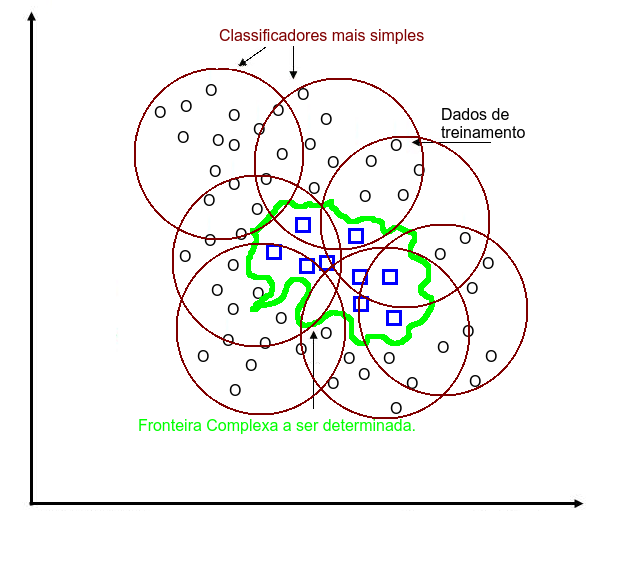
\includegraphics[width=8cm]{Imagens/Boost2.png}
\DeclareGraphicsExtensions.
\caption*{Fonte: Autor ``adaptado de'' \citefloat{Polikar}}
\label{Fig:Boost2}
\end{figure}


	\subsection{HAAR-Adaboost}

Somando-se todos os valores de cores de uma imagem, de forma que cada o valor em cada posição será a soma de todos os pixels acima e a esquerda daquela posição e armazenando esses valores em um vetor bidimensional, é possível calcular rapidamente o valor médio da cor em qualquer retângulo da imagem. Isso é feito subtraindo o valor encontrado no topo à esquerda do valor encontrado no fundo a direita e dividindo pelo número de pixels do retângulo. 

Segundo \citeonline{Xue}, outra particularidade dessa técnica é o tamanho da amostra. O tamanho da amostra se refere ao tamanho padrão de entrada dos classificadores de uma amostra de uma determinada imagem. As amostras são trechos retirados da imagem que possuem um determinado tamanho padrão. A imagem de origem é rotacionada aleatoriamente em volta de todos os eixos. Então pixels que possuem a intensidade dentro de um intervalo específico são interpretados como transparentes. Um ruído branco é adicionado às intensidades do plano de frente. A imagem obtida é então colocada dentro de um plano de fundo arbitrário proveniente do arquivo de descrição de fundos, redimensionada para a largura e altura desejados e então armazenadas em um vetor.

Muitos pesquisadores têm observado que adicionar mais classificadores fracos pode reduzir o erro de treinamento, mas dificilmente reduz o erro de generalização \cite{LiZhang} \cite{Brubaker} \cite{Mita}. Segundo \citeonline{Sakrapee} o desempenho da detecção decai drasticamente no estágios mais avançados da cascata, além disso, o desempenho da detecção usando características simples e únicas não são suficientemente discriminantes para separar imagens de faces das imagens onde faces não estão presentes. 

\citeonline{Mita} afirma que o uso da co-ocorrência de características em cada classificador fraco demonstrou um desempenho de classificação melhor do que se fossem utilizadas características simples. Assim, \citeonline{Sakrapee} propõe aplicar o conceito de unir características para criar a co-ocorrência de características. 

A contagem de amostras positivas \(N_{\text{AmostrasPositivas}}\) é um parâmetro muito importante, sem o qual o treinamento pode apresentar alguns erros ou pode nem mesmo prosseguir \cite{Mita}. Isso ocorre porque algumas amostras já utilizadas anteriormente por estágios já executados já podem ter sido classificadas isso pode manter o classificador em um mínimo local, a cada estágio a contagem de amostras positivas diminui até se tornar insuficiente. Para solucionar isso \citeonline{Maria} propôs o seguinte:

Suponha que um subconjunto de amostras positivas de tamanho \(N_{\text{AmostrasPositivas}}\) foi selecionado para treinar no estágio i, com i começando em zero, e \(Min_{\text{TaxaAcerto}}\) é a constante de treinamento para cada estágio.

Após treinar o estágio atual, pelo menos \(Min_{\text{TaxaAcerto}}\) * \(N_{\text{AmostrasPositivas}}\) amostras desse subconjunto devem passar por esse estágio, ou seja, o estágio atual da cascata com i+1 estágios tem que reconhecer a quantidade \(Min_{\text{TaxaAcerto}}\) das amostras selecionadas como positiva. Algumas amostras já utilizadas anteriormente por estágios já executados já podem ter sido classificadas como plano de fundo, mas não mais que ((1 - \(Min_{\text{TaxaAcerto}}\)) * \(N_{\text{AmostrasPositivas}}\)) em cada estágio. Veja equação ~\ref{eq1} onde, \(N_{\text{ImagensPositivas}}\) é a quantidade de imagens positivas total.

A equação ~\ref{eq2} foi usada para determinar o parâmetro \(N_{\text{AmostrasPositivas}}\).

\begin{equation}
\label{eq1} 
Amostras = ( N_{\text{Estágios}} - 1 ) * (1 - Min_{\text{TaxaAcerto}})
\end{equation} 

\begin{equation}
\label{eq2}
\begin{aligned}
N_{\text{ImagensPositivas}} = & [ N_{\text{AmostrasPositivas}} + Amostras * N_{\text{AmostrasPositivas}} ] + N_{\text{ImagensNegativas}} \\
			& \\
        		& \therefore  N_{\text{AmostrasPositivas}} = \frac { N_{\text{ImagensPositivas}} - N_{\text{ImagensNegativas}} } { 1 + Amostras} 
\end{aligned}
\end{equation}



A contagem de amostras do vetor que pode ser reconhecida como plano de fundo imediatamente é a variável \(N_{\text{ImagensNegativas}}\) na equação ~\ref{eq2}. 

\citeonline{Kuranov} afirmam que um tamanho de amostra de 20x20 pixels atingiu a maior taxa de acerto para detecção de faces. A cascata de classificadores foi implementada em formato de árvore, de forma que os ramos da árvore pudessem se dividir em 2 ou mais nós. \citeonline{Kuranov} afirmam também que para um tamanho de amostra de 18x18 e quatro nós de separação na fase de cascata tiveram um desempenho bom, enquanto para 20x20, dois nós a técnica teve um desempenho ligeiramente melhor, sendo a vantagem de desempenho entre usar 2, 3 ou 4 nós de separação nos classificadores fracos é menor do que a sua superioridade em relação a percorrer seus ramos. Sendo uma técnica usada para determinação de objetos o Haar-Adaboost será utilizado para identificar robôs da mesma forma que o HOG-SVM, de forma que uma comparação possa apontar qual deles se aplica nos robôs desenvolvidos.



\section{Controle Servo-Visual}

O controle servo-visual é uma técnica que usa o retorno de dados extraídos de um sensor de visão para controlar o movimento do robô. Esse tipo de controle, para o domínio RoboCup, se restringe ao controle dos dois servo-mecanismos referentes à cabeça do robô, mais especificamente do pescoço.

Uma das primeiras abordagens referentes ao controle servo-visual foi publicado por \citeonline{Corke}.Trabalhos mais recentes foram publicados por \citeonline{VS1} e por \citeonline{VS2}, aqui de uma forma mais abrangente no qual entende-se por controle servo-visual todas as ações feitas pelo robô que possuem como origem a visão do mesmo, inclusive movimentos das mãos, pés, rodas e articulações.

Técnicas de controle servo visual são classificados nos seguintes tipos:
\begin{enumerate}
     \item Baseada em Imagem (IBVS)
     \item Baseado Posição / Pose  (PBVS)
     \item Abordagem Híbrida
\end{enumerate}

A IBVS foi proposta por \citeonline{Weiss}. A lei de controle é baseada no erro entre as características atuais e desejadas no plano da imagem e não envolve qualquer estimativa da pose do alvo. Os recursos podem ser as coordenadas de recursos visuais, linhas ou momentos de regiões. A IBVS tem dificuldade com movimentos muito grandes, como rotações, o que veio a ser chamado retiro de câmera. \footnote{Do inglês: "Camera Retreat"}

A PBVS é uma técnica baseada em uma única câmera. Isto porque a posição do objeto de interesse é estimada em relação à câmera e, em seguida, é emitido um comando para o controlador de robô, que por sua vez, controla o robô. Neste caso, as características da imagem são extraídas mas, são, também, utilizadas para estimar a pose do objeto no espaço cartesiano.

Abordagens híbridas usam uma combinação dos controles previamente descritos. De forma geral, essas duas técnicas são consideradas passivas já que aguardam os dados do sensor de visão para tomar alguma decisão. 

Uma outra forma de encarar esse desafio é usar uma visão ativa, como proposta por \citeonline{Sharma}, que, de fato, procura ativamente o objeto a ser identificado e para tanto precisa tomar algumas decisões, mesmo que não haja dados relevantes vindos da câmera. 

Um sistema de visão ativo é capaz de interagir com o seu meio ambiente \cite{Tsotsos}, alterando o seu ponto de vista em vez de observá-lo passivamente e operando em sequências de imagens, em vez de em um único quadro \cite{Walther}. Além disso, a capacidade de acompanhar fisicamente um alvo reduz o borrão de movimento, aumentando a resolução de destino para tarefas de nível mais elevado, tais como classificação  \cite{Walther}. 

O controle servo-visual armazena as posições de trajetória do objeto e, por meio de regressão, estima as próximas posições do mesmo.  	Usando um algoritmo guloso encontra-se o melhor movimento antecipado da câmera em direção ao objeto. Para garantir um movimento plausível da câmera, é necessário considerar a cinemática e a dinâmica desse movimento, otimizando a trajetória da câmera para que essa possa manter o objeto em seu campo de visão.

Uma das vertentes da visão ativa é a configuração escravo-mestre \cite[p.2]{Fernandez}, no qual uma câmera está fixa e outra está em movimento. Ambas precisam estar em um mesmo sistema de coordenadas para que as informações trocadas entre elas sejam facilmente interpretadas. Essa configuração poderá ser usada em um projeto futuro, no qual o goleiro exerça o papel de câmera estática de supervisão enquanto os outros jogadores seriam as câmeras ativas em movimento. 

\section{Identificação de objetos}

% INTRODUÇÃO
Atualmente a visão computacional aplicada à robótica melhora no mesmo ritmo que a capacidade computacional. A quantidade de informação que uma imagem pode ser redundante ou desnecessária. Dessa forma o sistema de percepção deve reduzir ou tratar essa informação para que os objetivos sejam alcançados. 

Diversas abordagens têm sido propostas para o reconhecimento de objetos, sendo as mais recentes se valendo do uso de Redes Neurais Profundas (DNN) \cite{Deep1} \cite{Deep2} \cite{mccannobject}. A maioria usa uma ou mais características, geralmente únicas a esse objeto, fazendo-o sobressair aos demais itens na imagem capturada. Um ponto em comum às muitas das abordagens, decorre do uso de câmeras estáticas, nesse sentido o sistema poderia interpretar os dados provenientes da(s) câmera(s) de forma equivocada, já que a vibração da câmera causada pelo movimento do robô causa o borramento da região de interesse e arredores além de, provocar o movimento de pixels não pertencentes à essa região. 

Para reconhecer um objeto é necessário distinguí-lo do plano de fundo usando suas características únicas ou informação temporal, verificando quadro a quadro a região de interesse.

Com a finalidade de inferir algum formato à região de interesse, muitos algoritmos são propostos para a detecção de borda, incluindo o uso de gradientes. Reconhecer objetos parcialmente observáveis, em tempo real, torna-se uma tarefa particularmente difícil de  solucionar, já que um objeto parcialmente ocluso tem seu formato alterado. 

De forma análoga, a cor pode ser usada como uma forma de segmentar a região de interesse, que apesar de ser uma característica simples de se computar, é muito influenciada pela iluminação do ambiente. O time AUTMan, da Politécnica de Teerã \cite{AUTMan}, separa a imagem em três camadas, em cada qual segmenta uma cor referente à um objeto, sendo que cada uma dessas camadas serve de entrada para a próxima. Primeiramente as linhas de campo são segmentadas, em seguida o gol e por último, a bola. Dessa forma não é possível ver a bola se a segmentação do campo não estiver concluída. 

Todos os times participantes da Robocup são unânimes quanto ao uso de uma tabela de pesquisa (Look-up Table - LUT), na qual diversos valores de cor são armazenados previamente para uso na segmentação. Alguns times usam uma GUI (Graphical User Interface), Interface gráfica para Usuário para calibrar esses valores durante a competição.

\subsection{Reconhecimento da Bola}

Devido a importância da bola em jogo de futebol, o algoritmo de identificação da bola precisa ser rápido, robusto à oclusão e às diversas condições de iluminação. Algumas características da bola, como seu formato circular, sua cor e seu tamanho, são largamente utilizadas por todos os times, não só para encontrar a bola mas, também, para calcular sua distância do robô. 

%Como premissa, a bola apresentada em 2014 possuía cor predominantemente laranja, porém, devido ao seu polimento a mesma refletia uma certa quantidade de luz branca provenientes das luminárias.  

O filtro de Kalmann \cite{Kalmman} e o filtro de partículas proposto por \citeonline{AdaptPart}, também chamado de algoritmo de condensação  \cite{Condensation} para uso em imagens digitais, são amplamente usados em outros domínios como formas probabilísticas de inferir a posição de um objeto digital. São técnicas mais custosas em termos de tempo de computação mas, com mais poder de processamento, seria possível usá-las como uma forma complementar de identificar a posição na qual a bola se encontra.
 
Calcular a distância da bola ao robô, quando esta encontra-se parcialmente oclusa, adiciona uma componente de dificuldade, já que o tamanho conhecido da bola é usado como forma de computar essa distância. Nesse sentido, o time NUBots, da universidade de Newcastle \cite{Bunden}, criou linhas de varredura horizontais e verticais onde todos os pixels são considerados de forma individual. Determinam a linha de horizonte verde e, usando uma LUT, geram as transições referentes à classe de cor da bola. 

Esse mesmo time lidou com o problema da oclusão em 2012, adicionando uma etapa de verificação, onde quatro pontos de interesse, sem oclusão, podem ser usados em um método de atualização de centro, quando um determinado limite (threshold) de pixels consecutivos não pertencentes à bola são alcançados. Apesar de robusto contra ruído e alguma oclusão, esse método ainda precisa de duas verificações de tamanho e mais duas de cor. 

Esse algoritmo trabalha em baixo nível, segmentando pixels de forma individual e, por esse motivo, pode-se dizer que está efetuando a detecção com pouquíssimos recursos computacionais, infelizmente, trabalhando nesse nível, várias verificações precisam ser executadas de maneira que os pixels possam ser agrupados em regiões com uma mínima confiabilidade. A transformada de Hough probabilística usada pelo time Bold Hearts \citeonline{Bold}, da universidade de Hertfordshire, Inglaterra, parece fornecer essa confiabilidade ao custo de mais processamento. Nenhum time parece ter usado a informação temporal da câmera. Na verdade, o processamento aparenta ter sido efetuado como se tirassem diversas fotos e cada foto tivesse sido processada individualmente, sem que a informação do quadro anterior passasse para o próximo quadro.

Segmentar uma região por movimento é feito, de maneira geral, comparando os pixels do quadro atual com os pixels do quadro anterior, de forma individual ou em forma de máscaras. O rastreamento por fluxo ótico \cite{Fleet} funciona muito bem para câmeras estáticas onde os pixels que representam o plano de fundo tem pouca ou nenhuma alteração são facilmente subtraídos, deixando apenas os pixels que podem significar um objeto em movimento. Para o robô proposto, a câmera se movimenta e oscila frequentemente fazendo com que essa técnica apresente regiões provenientes de falsos movimentos, visto que, se a câmera inteira se mover muitos pixels que deveriam ser considerados parte do plano de fundo se moverão também.


\subsection{Identificação dos Robôs}
% RECONHECIMENTO DOS ROBÔS

Um importante item de um jogador de futebol é saber se seu adversário está a caminho de roubar-lhe a bola, ou saber a posição de seu companheiro de equipe para efetuar um passe. A identificação de robôs é especialmente difícil já que a variedade de robôs da liga é grande e a cada ano esses são modificados por suas equipes. Na verdade, na liga nenhum time demonstrou em seu trabalho de descrição de times qualquer menção ao reconhecimento de robôs.

O maior problema do algoritmo de reconhecimento de robôs é executá-lo em tempo real, devido ao número de dimensões ou características dos robôs e do fundo serem consideravelmente elevados, assim como, seus custos computacionais. Devido ao exposto, deve haver uma redução de características menos importantes. Na verdade o problema de reconhecimento dos robôs pode ser dividido em três partes:

\begin{itemize}
\item{Redução de características com a extração dos descritores mais relevantes;}
\item{Treinamento e classificação (É robô ou não é robô);}
\item{Identificação do time pela sua respectiva cor. (Sorteada no começo da partida)}
\end{itemize}

Um dos mais populares e bem sucedidos detectores de pessoas é o Histograma de Gradientes Orientados  \footnote{HOG - Do inglês: "Histogram of Oriented Gradients"}, usado juntamente com o classificador Máquina de Vetores de Suporte \footnote{SVM - Do inglês: "Support Vector Machine"}.

\citeonline{Castro} utilizaram essa abordagem com uma segmentação de cores para identificar a qual time cada robô pertence após um reconhecimento do torso do robô NAO \cite{NAO}\footnote{TDP - Do inglês: "Team Description Papers"}. Na standard platform league, todos os robôs obedecem ao padrão NAO, portanto se faz necessário identificar apenas um robô, e todos os outros terão o mesmo formato. Decorre do treinamento mais um problema dessa aplicação, a variedade de robôs presentes na categoria KidSize pode dificultar esse objetivo.

Há outros algoritmos que poderiam ser usados, como o Centrist \cite{Wu}. Outros detectores usam o movimento para iniciar o rastreamento e, como já foi visto, a câmera na cabeça do robô vibra muito. Outros classificadores como o LBP \cite{Viola}, o PCA/LDA \cite{Martinez}, entre outros, podem ser usados já que a classificação ocorre comparando vetores de descritores de treinamento com vetores de teste.

\begin{table}[ht!]
    \caption{Quadro de referência} \label{tbl:Times}
    \centering
    \begin{tabular}{|c|c|c|c|c|c|c|}
    \hline 
    Time 	& Sistema 	& Segmen  	& Bola		& Gol 		   & Linhas	   & Robô	\\ 
    	 	& Cores   	& tação		& 		&     		   & Campo	   & 	 	\\ 
    \hline 

    CIT 	& RGB - HSV 	& LUT	  	& Transição	&  Transição	   & Segmentação   & --	     	\\
    Brains	& 	 	& 	  	& de pixels	&  de pixels	   & Branco com    &	     	\\
    		& 	 	& 	  	& 		&  	 	   & Verificação   &	     	\\
    		& 	 	& 	  	& 		&  	 	   & Linear        &	     	\\

    \hline 

    Bold 	& RGB - HSV 	& LUT	  	& Transição	&  Transformada	   & Segmentação   & --     	\\
    Hearts	& 	 	& 	  	& de pixels	&  Hough 	   & Branco e      &	     	\\
    		& 	 	& 	  	& 		&  Probabi-  	   & Regressão     &	     	\\
    		& 	 	& 	  	& 		&  -lística	   & Linear        &	     	\\
    \hline 

    Baset	& RGB - HSV 	& LUT	  	& Transição	&  Transição	   & Segmentação   &            \\
    		& 	 	& 	  	& de pixels	&  de pixels	   & Branco        & --     	\\
    		& 	 	& 	  	& Contornos	&  Contornos       & RANSAC        &	     	\\
    \hline 

    Eros	& YUYV  	& LUT	  	& Transição	&  Transformada	   & Segmentação   & --	     	\\
    		& nativo	& 	  	& de pixels	&  de Hough	   & Branco        &	     	\\

    \hline 
     
    AUTMan	& RGB - HSV 	& LUT	  	& Transição	&  Transição	   & Segmentação   & --	     \\
    		& 	 	& 	  	& de pixels	&  de pixels       & Branco        &	     \\
    \hline

    \end{tabular}
    \caption*{Fonte: Artigos de Descrição de Equipes$^4$, 2014 \cite{AUTMan}, \cite{Bold}, \cite{CIT}, \cite{Baset}, \cite{EROS} }

\end{table}

\section{Considerações finais}

Vimos nesse capítulo que as equipes, inseridas no domínio RoboCup, trabalham em baixo nível e em médio nível \cite{AUTMan}, \cite{Bold}, \cite{CIT}, \cite{Baset}, \cite{EROS}. Essas técnicas são bem utilizadas e têm resultados pertinentes porém, com a mudança das regras, esses algoritmos vão precisar de cada vez mais estágios de verificação. Vimos também que diversas adversidades são inerentes do domínio, e que por esse motivo precisam de técnicas que possam identificar características, mas, que também, possam levar em conta algum contexto do objeto pertencente ao jogo.
Dessa forma, ao lançar o artifício de utilizar técnicas de alto nível e considerando o que outras equipes têm feito, serão abordados no próximo capítulo dois aspectos do sistema de visão: 

\begin{enumerate}
	\item a identificação e rastreamento da bola.
		\begin{enumerate}
			\item Algoritmo proposto conforme algoritimo ~\ref{lst:algBall}
			\item Descritor e Classificador Haar-AdaBoost
		\end{enumerate}
	\item a detecção de robôs.
		\begin{enumerate}
			\item Descritor e Classificador HOG-SVM
			\item Descritor e Classificador Haar-AdaBoost
		\end{enumerate}
\end{enumerate}

Nos dois casos, as técnicas serão postas a prova com o mesmo conjunto de imagens pertinentes aos seus respectivos objetivos. De maneira que possam coexistir no sistema de visão do robô sem onerá-lo em demasia.








%*********************************************************************************************************************************************
%---------------------------------------------------------------------------------------------------------------------------------------------
%---------------------------------------------CAPÍTULO 3 - TRABALHO CORRELATOS----------------------------------------------------------------
%---------------------------------------------------------------------------------------------------------------------------------------------
%*********************************************************************************************************************************************

%\chapter{Visão Computacional Aplicada a Robótica - Domínio RoboCup Humanoide}
%\label{chap:relatedwork}
%No embasamento teórico, no capítulo 2, foi feita uma revisão bibliográfica de alguns algoritmos de visão computacional bem conceituados, além de, o que outras equipes têm feito com esses algoritmos no sentido de solucionar os problemas visuais do jogo de futebol. Utilizando o conhecimento desse capítulo, a proposta desse trabalho tem por objetivo criar um sistema de visão rápido e eficaz, abordando o uso dessas técnicas no domínio proposto. Visando facilitar o entendimento de suas diversas aplicações, as seções a seguir foram sub-divididas em: \ref{Bola}, que lida com as propostas escolhidas para o rastreamento da bola. A seção \ref{Robos} apresenta a proposta para a detecção de robôs (companheiros ou adversários). A seção \ref{Servo} trata do controle dos servo-mecanismos pan-tilt e como cada um dos algoritmos podem controlá-lo em um determinado instante de tempo. E, finalmente, a seção \ref{Sistema} propõe como todos esses algoritmos estariam interligados.

\section{Bola}
\label{Bola}

A bola tem características próprias, que podem ser usadas para identificá-la, além de outras duas informações que são do campo, de fundo verde, e estar abaixo da linha do horizonte, entenda-se por linha do horizonte pela linha mediana da imagem de captura quando a câmera está posicionada paralelamente ao plano transversal do robô e paralelo ao piso. Ver figura ~\ref{Fig:Ori} para referência sobre o plano transversal.

\begin{figure}[!h!]
\centering \caption{Planos que cortam o ser humano utilizados em robôs humanoides.}
\includegraphics[width=5cm]{Imagens/Orientation.png}
\DeclareGraphicsExtensions.
\caption*{Fonte: Parte integrante do livro \citefloat{bookFeedbackcontrol}.}
\label{Fig:Ori}
\end{figure}

Na verdade, nenhum robô da liga é capaz de erguer a bola, isso quer dizer que, os robôs atualmente desenvolvidos ainda não chutam a bola de forma a erguê-la mais que alguns centímetros do chão, assim é razoável estimar que a bola estará sempre abaixo da linha do horizonte, tipicamente envolta por uma região verde com a matiz entre 190 e 270 graus. Isso irá evoluir gradativamente e significará uma quebra de paradigma para o rastreamento da bola, que não será abordado neste trabalho de pesquisa. 

O rastreamento clássico, usando o fluxo ótico de pixels \cite{Faria}, falha nessa aplicação devido à trepidação da câmera e também ao fato dela não estar fixa em um determinado ponto do campo. O quadro adquirido da captura da câmera é inserido no sistema de rastreamento da bola e é uma variável bloqueada via mutex. Esse bloqueio permite que diversos processos paralelos acessem a captura da câmera sem modificá-la, o que inviabilizaria o uso dessa imagem por vários processos de forma paralela. 

A ideia aqui é começar fazendo um pré-processamento da imagem transformando o sistema de cores do RGB para o HSV, isso é especialmente importante, já que o HSV possui uma certa robustez à mudanças de iluminação. 

Duas abordagens serão comparadas, uma usando segmentação e outra usando a técnica HAAR-AdaBoost para reconhecimento de objetos.
Para a bola laranja a abordagem de segmentação e círculos de Hough com a imagem devidamente pré-processada e utilizando a técnica HAAR-AdaBoost para a detecção da bola branca. Dividindo a resolução da tela em nove regiões, é possível inferir de forma qualitativa se a bola está à direita, esquerda e, de forma quantitativa calculando valores de distância. Isso será melhor explicado na seção que trata do controle servo-visual Pan-tilt na seção ~\ref{Servo}.

\subsection{A Bola Laranja}

No caso da bola laranja, após segmentação usando uma LUT (Look-Up Table), duas operações morfológicas, Dilatação e Erosão, são aplicadas, ambas para retirar áreas e ruídos que não fazem parte da região de interesse. Ao mover-se pelo campo de visão do robô a bola provoca um borramento em sua imagem, para minimizar esse borramento aplica-se uma suavização usando uma Gaussiana. A transformada de Hough para círculos é aplicada e, com isso, temos a posição do centro da bola e seu raio expressos em pixels.Note que a bola usada em 2014, figura ~\ref{Fig:BolaLaranja}, é lisa em termos construtivos, chegando inclusive a refletir a luz branca, porém, em termos de cor possui uma heterogeneidade bem marcante.

\begin{figure}[!h!]
\centering \caption{A bola utilizada em 2014.}
\includegraphics[width=7cm]{Imagens/ImBolaL.png}
\DeclareGraphicsExtensions.
\caption*{Fonte: Autor.}
\label{Fig:BolaLaranja}
\end{figure}



\begin{algorithm}[!h!]


\caption{Algoritimo de rastreamento da bola laranja - Círculos de Hough.}\label{lst:algBall}


\Entrada{Abra Captura da Câmera (Dispositivo 0)}
\Se{Captura vazia}
	{Erro! Dispositivo não está pronto.
	Aborte Algoritimo.
		}

\Enqto{ Não for pressionada a tecla esc e Quadro não vazio}
{

Extraia um quadro RGB da captura, converta para uma imagem HSV.

\begin{equation}
     \centering
    	H = \left\{
		\begin{array}
		{ccl} 
		$$\theta, 	& Se B  \leq  G $$\\
		$$360 - \theta,	& Se B  >  G $$
		\end{array} 
\right.
\end{equation}

\begin{equation}
	\theta  =  \cos^-{^1} \left[  {   \frac {  \frac {1} {2} * [(R -G) + (R-B)]}  {  \sqrt{[(R -G)^2 + (R -B)(G -B)]}   }    }\right]
\end{equation}

\begin{equation}
	S  =  1 - { \frac {3} {(R+G+B)} } * [min (R,G,B)]
\end{equation}

\begin{equation}
	I  =  { \frac {1} {3}} * {(R+G+B)}
\end{equation}



\Entrada{Tabela de pesquisa (LUT). (0<H<35, 0<S<180, 0<V<255)}

\ParaTodo {Pixel dentro da imagem HSV e dentro dos limites da LUT}
	{Altere o valor do Pixel de uma matriz binária na mesma posição}

Na matriz binária aplique Erosão seguida da Dilatação. ( 5x5 Pixels)

Aplique filtro espacial. (Gaussiana 9x9 Pixels)

Transformada de Hough para círculos:

- Atualize a média móvel do raio (MRB) e da posição XY dos círculos encontrados.

\begin{equation} 
	D_{bola} = \frac {9143} {MRB}
\end{equation}\\

Armazene \(D_{bola}\), a posição dos servos Pan-Tilt em graus e da bola em pixels.
}

\Retorna \(D_{bola}\)

\Comment*[h]{\begin{center}  \begin{localsize}{12} \textrm{Fonte: Autor} \end{localsize} \end{center}}



\end{algorithm}%%


A fim de incorporar a informação temporal, os centros dos círculos e raios encontrados serão armazenados na forma de média móvel (Ver referência de séries temporais no “ANEXO A”, trecho do trabalho de \citeonline{Lopes}). Isso é importante para melhorar a estimativa da posição da bola. Essa média garante que a bola estará em uma posição muito próxima de sua última detecção. Como o tamanho da bola é conhecido, podemos achar uma relação entre o tamanho real em centímetros e o tamanho da bola em pixels, dada a resolução da tela.

Na medida que a bola se afasta, seu tamanho em pixels se reduz até o momento que o algoritmo acaba tratando-a como ruído, nesse momento a ideia é utilizar o algoritmo de condensação, a fim de, tentar inferir sua posição de forma qualitativa se está a direita ou a esquerda no campo de visão do robô. Infelizmente seu tamanho não será calculado até que o robô se aproxime novamente da bola. Perceba aqui que, para distinguir a bola do plano de fundo, a cor foi utilizada como característica antes do formato, isso foi feito, visando diminuir o espaço de ação da transformada de Hough para círculos, tornando-a mais rápido. Veja algoritimo ~\ref{lst:algBall} proposto. 

No capítulo 2 fica claro que a transformada de Hough para círculos testa todas as possibilidades de círculo para todos os pixels encontrados usando três parâmetros, dessa forma, se esse algoritmo fosse aplicado à toda a imagem, provavelmente o algoritmo ficaria mais robusto porém, às custas de mais processamento.

\subsection{A Bola Branca}

A modificação do regulamento da competição fez com que todas as equipes tivessem que pensar em uma forma diferente de reconhecer a bola. A bola branca da figura ~\ref{Fig:BolaBranca}, diferentemente da usada anteriormente, possui uma textura que pode ser usada como característica discrepante. Assim, a proposta é o descritor HAAR com o classificador AdaBoost, onde diversas imagens serão coletadas com a própria câmera do robô. A bola será posicionada em diferentes distâncias e posições no campo de futebol, essas imagens denominadas imagens positivas possuem a bola em qualquer posição da imagem. A bola se encontrará por completo na imagem, isso quer dizer que não haverá oclusão nas imagens de treinamento.


\begin{figure}[!h!]
\centering \caption{A bola utilizada em 2015.}
\includegraphics[width=8cm]{Imagens/ImBola.png}
\DeclareGraphicsExtensions.
\caption*{Fonte: Autor.}
\label{Fig:BolaBranca}
\end{figure}

As imagens negativas são adquiridas rotacionando o robô em diversas posições do \\campo de futebol. Imagens de multidões também foram usadas. Isso é feito para que se possua uma visão 360 graus do campo e para que de qualquer posição do robô o mesmo possa identificar um plano de fundo negativo, mesmo com muitas pessoas em volta e aumenta a probabilidade de que a bola será encontrada nessas condições. 

\begin{algorithm}

\caption{Algoritmo de Identificação da bola branca. (HAAR-Adaboost Offline)}\label{lst:algHaarOFBall}

\Entrada{Conjunto de imagens positivas - Contém robôs participantes}
\Entrada{Conjunto de imagens negativas - Não contém robôs}

\Entrada{Posição da bola contida em todas as imagens positivas}

\ParaTodo {Estágio da árvore e para todas as imagens}
{
\Enqto{\(Min_{\text{TaxaAcerto}}\) = 0,999 não atingida}
	{
	Extraia as características de HAAR para as imagens positivas.\\
	Execute o Adaboost conforme algoritmo ~\ref{lst:algHaar} usando como parâmetros:\\
		- Tamanho da amostra = 20x20 Pixels;\\
		- Tamanho mínimo do objeto = 30x30 Pixels;\\
		- Tamanho máximo do objeto = Resolução vertical x \( \frac {Resolução Horizontal}{2}\) Pixels\\
		- Classificador 8 Vizinhos mais próximos. \\
	}
	Armazene a hipótese final do estágio.\\
}
	Armazene a hipótese final em um arquivo .xml


\Comment*[h]{\begin{center}  \begin{localsize}{12} \textrm{Fonte: Autor ``Adaptado de'' \citefloat{Adaboost}} \end{localsize} \end{center}}


\end{algorithm}

Tanto o algoritimo de treinamento ~\ref{lst:algHaarOFBall}, quanto o de identificação online ~\ref{lst:algHaarOnBall}, estão sendo propostos utilizando-se os parâmetros de seus respectivos artigos originais, mas alguns parâmetros serão postos a prova no capítulo ~\ref{chap:experiments}.

\begin{algorithm}

\caption{Algoritmo de Identificação da bola branca. (HAAR-Adaboost Online)}\label{lst:algHaarOnBall}

\Entrada{Árvore proveniente do Adaboost (Arquivo .xml)}

\Entrada{Aquisição da câmera}

\Enqto{ Quadro não vazio}
{

Extraia o vetor de caracterísiticas (descritores) da imagem adquirida.\\
Percorra os nós (Estágios) da árvore presentes no arquivo xml encontrando a melhor classificação para a imagem adquirida\\

	\Se {Houver bola presente na imagem}
	{
		Para cada bloco da imagem adquirida, encontre em qual bloco a bola se encontra\\

		Calcule seu raio em pixels\\

		Armazene o centro do círculo e a raio em pixels\\

		Calcule sua distância real até o robô em centímetros\\
	}
}



\Comment*[h]{\begin{center}  \begin{localsize}{12} \textrm{Fonte: Autor ``Adaptado de'' \citefloat{Adaboost}} \end{localsize} \end{center}}


\end{algorithm}

Como forma de checar o qualidade do classificador uma curva ROC será plotada e como forma de verificar o desempenho será usada a taxa de quadros por segundo após processamento para a resolução de 1920x1080 pixels. Essa resolução foi escolhida devido ao seu potencial de alcance de detecção da bola, já que existe uma correlação entre o tamanho da mesma em pixels e sua distância da câmera.


\section{Adversários e Companheiros de Equipe}
\label{Robos}

A ideia geral é identificar objetos conhecidos e parecidos com relação à alguma característica. Com os robôs não seria diferente, entretanto, existem poucas características semelhantes entre os robôs da liga. Na verdade, mesmo que muitas equipes ainda usem uma plataforma (Darwin-OP) \cite{Darwin} com algumas modificações, os robôs, de maneira geral, têm formas e tamanhos variados, veja figura ~\ref{Fig:DivRob},  e identificar esses robôs de forma confiável é complexo. 

Os descritores HOG e HAAR e seus classificadores em sua forma clássica, respectivamente, SVM e AdaBoost serão testados para a identificação dos robôs em campo. 


\begin{figure}[!h!]
\centering \caption{A diversidade de robôs da liga humanoide.}
\includegraphics[width=15cm]{Imagens/liga.jpg}
\DeclareGraphicsExtensions.
\caption*{Fonte: Autor.}
\label{Fig:DivRob}
\end{figure}

Ambos os descritores são computados para todas as imagens de um conjunto de imagens positivas e negativas, entenda-se imagens positivas, como sendo imagens que possuam apenas um robô em qualquer pose e em diversos cenários. 
Esses vetores de descrição são inseridos em seus respectivos classificadores, sendo esse treinamento efetuado em um computador externo ao robô com as mesmas especificações. O classificador treinado é inserido no robô, que, durante o jogo, calcula o descritor de um quadro adquirido e classifica o vetor de descrição no classificador treinado. A resposta do classificador informa se há robô no quadro e qual região tem a maior quantidade de descritores, apontando em qual região o robô foi identificado na imagem. Os algoritimos propostos [~\ref{lst:algROF}] [~\ref{lst:algROn}] [~\ref{lst:algHaarOF}] [~\ref{lst:algHaarOn}] são apresentados conforme revisão feita nos capítulos anteriores.

O mesmo conjunto de imagens positivas e negativas serão computadas tanto pelo HAAR com o AdaBoost como pelo HOG com o SVM, de forma que seja possível definir qual possui maior precisão, com maior taxa de quadros por segundo após processamento, para o robô proposto.
\begin{algorithm}
{
\caption{Algoritmo para Identificação de Robôs. (HOG-SVM Offline)}\label{lst:algROF}

\Entrada{Conjunto de imagens positivas - Contém robôs participantes}
\Entrada{Conjunto de imagens negativas - Não contém robôs}

Extraia, do diretório de imagens negativas, todas as imagens que possuam tamanho e extensão compatíveis (jpg,jpeg,png,bmp)

Calcule o histograma de gradientes para todas as imagens.

Armazene o vetor de características (descritores) de cada uma das imagens negativas.

Extraia, do diretório de imagens positivas, todas as imagens que possuam tamanho e extensão compatíveis (jpg,jpeg,png,bmp)

Calcule o histograma de gradientes para todas as imagens desse diretório.

Armazene o vetor de características (descritores) de cada uma das imagens positivas.

Armazene o vetor de características (descritores) de cada uma das imagens negativas.

\Entrada{Vetores de características (descritores) das imagens positivas}
\Entrada{Vetores de características (descritores) das imagens negativas}

Determine os vetores de suporte e o hiperplano que melhor separa as duas classes usando o SVM.

\Entrada{Tabela com todas as alturas de todos os robôs de todos os times}
\Entrada{Tabela com a cor do time adversário}
}



\Comment*[h]{\begin{center}  \begin{localsize}{12} \textrm{Fonte: Autor ``Adaptado de'' \citefloat{Dallal}.} \end{localsize} \end{center}}

\end{algorithm}

\pagebreak

\section{HOG-SVM Online}

\begin{algorithm}

\caption{Algoritmo para Identificação de Robôs. (HOG-SVM Online)}\label{lst:algROn}

\Entrada{Hiperplano proveniente do SVM}
\Entrada{Aquisição da câmera}

\Enqto{ Quadro não vazio}
{
Calcule o histograma de gradientes da imagem adquirida da câmera

Extraia o vetor de caracterísiticas (descritores) da imagem adquirida.

Use o SVM para classificar o vetor de caracterísiticas da imagem adquirida.

	\Se {Houver robô presente na imagem}
	{
		Para cada bloco da imagem adquirida, encontre em qual bloco do histograma normalizado o robô se encontra\\

		Calcule sua altura em pixels\\

		Armazene o centro do bloco e a altura em pixels\\

		Segmentação da cor do time.\\

		Se a área na qual o robô for identificado conter o centroide referente à cor do time\\

		Busque na tabela de alturas qual a altura em centímetros do robô que foi identificado\\

		Calcule sua distância real até o robô em centímetros\\
	}

}

\Comment*[h]{\begin{center}  \begin{localsize}{12} \textrm{Fonte: Autor ``Adaptado de'' \citefloat{Dallal}.} \end{localsize} \end{center}}

\end{algorithm}

Com essas informações, a altura do robô em pixels e a informação de que existe pelo menos um robô na imagem, é necessário identificar a qual equipe o(s) robô(s) pertence(m). Para tal, usa-se a informação da cor da camisa via segmentação simples, ou seja, se a região, delimitada pela janela de detecção, onde foi identificado o robô coincidir com a região que possui uma área azul (ciano), esse é um robô pertencente ao time azul. As duas cores, azul ciano ou magenta, são sorteadas antes do início da partida. Com o(s) robô(s) identificado(s), é necessário calcular sua(s) distância(s) até o robô que está vendo a ação. Por se tratar de uma visão monocular, calcular a distância dos robôs necessita da informação de sua altura real assim, uma tabela de pesquisa é alimentada com as informações de altura de todos os robôs da liga em centímetros e, finalmente, com a altura do robô em pixels calculado no passo anterior e a altura real, é possível estimar a distância entre esses dois robôs.

\begin{algorithm}

\caption{Algoritmo de Identificação de robôs. (HAAR-Adaboost Offline)}\label{lst:algHaarOF}

\Entrada{Conjunto de imagens positivas - Contém robôs participantes}
\Entrada{Conjunto de imagens negativas - Não contém robôs}

\Entrada{Posição dos robôs contidos nas imagens positivas}

\ParaTodo {Estágio da árvore e para todas as imagens}
{
\Enqto{\(Min_{\text{TaxaAcerto}}\) = 0,999 não atingida}
	{
	Extraia as características de HAAR para as imagens positivas.\\
	Execute o Adaboost conforme algoritmo ~\ref{lst:algHaar} usando como parâmetros:\\
		- Tamanho da amostra = 20x20 Pixels;\\
		- Tamanho mínimo do objeto = 30x30 Pixels;\\
		- Tamanho máximo do objeto = Resolução vertical x \( \frac {Resolução Horizontal}{2}\) Pixels\\
		- Classificador 8 Vizinhos mais próximos. \\
	}
	Armazene a hipótese final do estágio.\\
}
	Armazene a hipótese final em um arquivo.
\Comment*[h]{\begin{center}  \begin{localsize}{12} \textrm{Fonte: Autor ``Adaptado de'' \citefloat{Adaboost}} \end{localsize} \end{center}}

\end{algorithm}

\begin{algorithm}

\caption{Algoritmo de Identificação de robôs. (HAAR-Adaboost Online)}\label{lst:algHaarOn}

\Entrada{Árvore proveniente do Adaboost (Hipótese Final)}

\Entrada{Aquisição da câmera}

\Enqto{ Quadro não vazio}
{

Extraia o vetor de caracterísiticas (descritores) da imagem adquirida.\\
Percorra os nós (Estágios) da árvore para a imagem adquirida\\

	\Se {Houver robô presente na imagem}
	{
		Na imagem encontre em qual bloco o robô se encontra\\

		Calcule sua altura em pixels\\

		Armazene o centro do bloco e a altura em pixels\\

		Segmentação da cor do time.\\

		Se a área na qual o robô for identificado conter a cor do time\\

		Busque na tabela de alturas qual a altura do robô que foi identificado\\

		Calcule sua distância real até o robô em centímetros\\
	}
}

\Comment*[h]{\begin{center}  \begin{localsize}{12} \textrm{Fonte: Autor ``Adaptado de'' \citefloat{Adaboost}} \end{localsize} \end{center}}

\end{algorithm}

\pagebreak

\section{Controle Servo-Visual}
\label{Servo}

O controle servo-visual toma atitudes ativas e reativas, procurando os objetos quando não estão em seu campo de visão, de forma ativa, e seguindo-os, de forma reativa, quando estão à vista. A proposta do controle servo-visual foi feita dividindo o quadro capturado pela câmera em nove regiões distribuídas da seguinte forma: três na horizontal e cada uma dessas regiões é novamente dividida em três, dessa vez na vertical. As regiões não são divididas igualmente. A região central é menor do que as outras oito regiões pois, seria o equivalente do ser humano ao foco principal da visão, ou visão central, e as outras seriam equivalentes à visão periférica.

Independentemente da região na qual o objeto de interesse se encontra, o controle de pan-tilt deve mover a cabeça do robô até levá-lo à região central, ver algoritimo ~\ref{lst:algCent}. Na figura ~\ref{Fig:Regioes} essa região se refere à região 5. 

\begin{figure}[!th]
\centering \caption{Divisão esquemática do quadro em 9 regiões.}
\includegraphics[width=3in]{Imagens/Regioes.png}
\DeclareGraphicsExtensions.
\caption*{Fonte: Autor}
\label{Fig:Regioes}
\end{figure}

O tamanho da região 5 é fundamental para o bom funcionamento do sistema. Se for muito pequena, o robô terá problemas ao centralizar o objeto que sairá muito facilmente dessa região, se o contrário for verdade, a cabeça do robô se movimentará muito pouco e o objeto não será centralizado corretamente. A proposta aqui é que a região 5 tenha 5\% da resolução da câmera nos dois eixos. 

\begin{algorithm}

\caption{Algoritmo para buscar e centralizar o objeto}\label{lst:algCent}

Divida o quadro de captura em 3 regiões horizontais, sendo a região central com 5\% da resolução horizontal.\\
Divida o quadro de captura em 3 regiões verticais, sendo a região central com 5\% da resolução vertical.\\
\Enqto{Quadro não vazio}
{
	\Se{Dentro do quadro houver objeto}
		{
		Encontre em qual região o objeto se encontra usando sua posição.\\
			\Se {O objeto estiver na região 5 (central)} 
					{Mantenha o objeto nessa região parando o movimento}
			\Se {O objeto estiver nas regiões 1, 4 e 7} 
					{Some a posição atual do servo com a quantidade de graus para o pan}
			\Se {O objeto estiver nas regiões 3, 6 e 9} 
					{Subtraia a posição atual do servo com a quantidade de graus para o pan}
			\Se {O objeto estiver nas regiões 1, 2 e 3} 
					{Some a posição atual do servo com a quantidade de graus para o tilt}
			\Se {O objeto estiver nas regiões 7, 8 e 9} 
					{Subtraia a posição atual do servo com a quantidade de graus para o tilt}
		Guarde posição dos servos\\
		}
		\Senao
		{		
		Chame algoritmo de busca \ varredura
		}
	
}
\Retorna \(Posicao do Servo\)

\Comment*[h]{\begin{center}  \begin{localsize}{12} \textrm{Fonte: Autor.} \end{localsize} \end{center}}


\end{algorithm}

Quando o objeto a ser procurado não estiver no campo de visão, um algoritmo de varredura entra em ação, varrendo em três diferentes níveis, na vertical começando em 0 graus, passando por -22,5 graus e finalmente -45 graus, enquanto movimenta a cabeça na horizontal da esquerda para a direita e da direita para a esquerda, em cada um desses níveis.


\section{O sistema de visão}
\label{Sistema}

A visão do robô, a ser desenvolvida, será um sistema com dois processos paralelos e dois sequenciais. Todos usarão um quadro disponível no momento de aquisição da câmera. Isso permitirá que todos os processos de visão adquiram informação do ambiente praticamente ao mesmo tempo.

Apenas um processo poderá ter controle sobre o Pan-Tilt em um determinado momento, isso, entretanto, não impedirá que os outros processos continuem a adquirir e processar as informações provenientes do ambiente, ver figura ~\ref{Fig:Start}. Haverá um atraso entre processos devido à diferença de complexidade entre as tarefas a serem executadas, isso se torna óbvio já que algumas são computacionalmente mais custosas do que outras. 


\begin{figure}[!t]
\centering \caption{Visão Geral do Software a ser Implementado.}
\includegraphics[width=5in]{Imagens/StartP.png}
\DeclareGraphicsExtensions.
\caption*{Fonte: Autor}
\label{Fig:Start}
\end{figure}


O que acontece é que a variável quadro é protegida por mutex, o bloqueio permite que apenas um dos processos utilize essa variável. Por exemplo, o algoritmo da bola é mais rápido que o de identificação de robôs, assim pode ser que o quadro disponível para reconhecimento de robôs seja diferente do que foi usado para rastreamento da bola. O mutex ou exclusão mútua, é um recurso técnico usado em programação paralela para evitar que dois processos tenham controle de um recurso que precisa ser compartilhado. O meio mais comum de se efetuar a exclusão mútua é através de um semáforo, que bloqueia o recurso para cada um dos processos liberando-o do processamento em seguida, de forma que no período de bloqueio apenas o processo definido pelo mutex pode controlar o recurso.



%*********************************************************************************************************************************************
%---------------------------------------------------------------------------------------------------------------------------------------------
%-------------------------------------------  CAPÍTULO 4 - PROPOSTA --------------------------------------------------------------------------
%---------------------------------------------------------------------------------------------------------------------------------------------
%*********************************************************************************************************************************************

\chapter{Sistema Desenvolvido}
\label{chap:software}
No embasamento teórico, no capítulo 2, foi feita uma revisão bibliográfica de alguns algoritmos de visão computacional bem conceituados, além de, o que outras equipes têm feito com esses algoritmos no sentido de solucionar os problemas visuais do jogo de futebol. Utilizando o conhecimento desse capítulo, a proposta desse trabalho tem por objetivo criar um sistema de visão rápido e eficaz, abordando o uso dessas técnicas no domínio proposto. Visando facilitar o entendimento de suas diversas aplicações, as seções a seguir foram sub-divididas em: \ref{Bola}, que lida com as propostas escolhidas para o rastreamento da bola. A seção \ref{Robos} apresenta a proposta para a detecção de robôs (companheiros ou adversários). A seção \ref{Servo} trata do controle dos servo-mecanismos pan-tilt e como cada um dos algoritmos podem controlá-lo em um determinado instante de tempo. E, finalmente, a seção \ref{Sistema} propõe como todos esses algoritmos estariam interligados.

\section{Bola}
\label{Bola}

A bola tem características próprias, que podem ser usadas para identificá-la, além de outras duas informações que são do campo, de fundo verde, e estar abaixo da linha do horizonte, entenda-se por linha do horizonte pela linha mediana da imagem de captura quando a câmera está posicionada paralelamente ao plano transversal do robô e paralelo ao piso. Ver figura ~\ref{Fig:Ori} para referência sobre o plano transversal.

\begin{figure}[!h!]
\centering \caption{Planos que cortam o ser humano utilizados em robôs humanoides.}
\includegraphics[width=5cm]{Imagens/Orientation.png}
\DeclareGraphicsExtensions.
\caption*{Fonte: Parte integrante do livro \citefloat{bookFeedbackcontrol}.}
\label{Fig:Ori}
\end{figure}

Na verdade, nenhum robô da liga é capaz de erguer a bola, isso quer dizer que, os robôs atualmente desenvolvidos ainda não chutam a bola de forma a erguê-la mais que alguns centímetros do chão, assim é razoável estimar que a bola estará sempre abaixo da linha do horizonte, tipicamente envolta por uma região verde com a matiz entre 190 e 270 graus. Isso irá evoluir gradativamente e significará uma quebra de paradigma para o rastreamento da bola, que não será abordado neste trabalho de pesquisa. 

O rastreamento clássico, usando o fluxo ótico de pixels \cite{Faria}, falha nessa aplicação devido à trepidação da câmera e também ao fato dela não estar fixa em um determinado ponto do campo. O quadro adquirido da captura da câmera é inserido no sistema de rastreamento da bola e é uma variável bloqueada via mutex. Esse bloqueio permite que diversos processos paralelos acessem a captura da câmera sem modificá-la, o que inviabilizaria o uso dessa imagem por vários processos de forma paralela. 

A ideia aqui é começar fazendo um pré-processamento da imagem transformando o sistema de cores do RGB para o HSV, isso é especialmente importante, já que o HSV possui uma certa robustez à mudanças de iluminação. 

Duas abordagens serão comparadas, uma usando segmentação e outra usando a técnica HAAR-AdaBoost para reconhecimento de objetos.
Para a bola laranja a abordagem de segmentação e círculos de Hough com a imagem devidamente pré-processada e utilizando a técnica HAAR-AdaBoost para a detecção da bola branca. Dividindo a resolução da tela em nove regiões, é possível inferir de forma qualitativa se a bola está à direita, esquerda e, de forma quantitativa calculando valores de distância. Isso será melhor explicado na seção que trata do controle servo-visual Pan-tilt na seção ~\ref{Servo}.

\subsection{A Bola Laranja}

No caso da bola laranja, após segmentação usando uma LUT (Look-Up Table), duas operações morfológicas, Dilatação e Erosão, são aplicadas, ambas para retirar áreas e ruídos que não fazem parte da região de interesse. Ao mover-se pelo campo de visão do robô a bola provoca um borramento em sua imagem, para minimizar esse borramento aplica-se uma suavização usando uma Gaussiana. A transformada de Hough para círculos é aplicada e, com isso, temos a posição do centro da bola e seu raio expressos em pixels.Note que a bola usada em 2014, figura ~\ref{Fig:BolaLaranja}, é lisa em termos construtivos, chegando inclusive a refletir a luz branca, porém, em termos de cor possui uma heterogeneidade bem marcante.

\begin{figure}[!h!]
\centering \caption{A bola utilizada em 2014.}
\includegraphics[width=7cm]{Imagens/ImBolaL.png}
\DeclareGraphicsExtensions.
\caption*{Fonte: Autor.}
\label{Fig:BolaLaranja}
\end{figure}



\begin{algorithm}[!h!]


\caption{Algoritimo de rastreamento da bola laranja - Círculos de Hough.}\label{lst:algBall}


\Entrada{Abra Captura da Câmera (Dispositivo 0)}
\Se{Captura vazia}
	{Erro! Dispositivo não está pronto.
	Aborte Algoritimo.
		}

\Enqto{ Não for pressionada a tecla esc e Quadro não vazio}
{

Extraia um quadro RGB da captura, converta para uma imagem HSV.

\begin{equation}
     \centering
    	H = \left\{
		\begin{array}
		{ccl} 
		$$\theta, 	& Se B  \leq  G $$\\
		$$360 - \theta,	& Se B  >  G $$
		\end{array} 
\right.
\end{equation}

\begin{equation}
	\theta  =  \cos^-{^1} \left[  {   \frac {  \frac {1} {2} * [(R -G) + (R-B)]}  {  \sqrt{[(R -G)^2 + (R -B)(G -B)]}   }    }\right]
\end{equation}

\begin{equation}
	S  =  1 - { \frac {3} {(R+G+B)} } * [min (R,G,B)]
\end{equation}

\begin{equation}
	I  =  { \frac {1} {3}} * {(R+G+B)}
\end{equation}



\Entrada{Tabela de pesquisa (LUT). (0<H<35, 0<S<180, 0<V<255)}

\ParaTodo {Pixel dentro da imagem HSV e dentro dos limites da LUT}
	{Altere o valor do Pixel de uma matriz binária na mesma posição}

Na matriz binária aplique Erosão seguida da Dilatação. ( 5x5 Pixels)

Aplique filtro espacial. (Gaussiana 9x9 Pixels)

Transformada de Hough para círculos:

- Atualize a média móvel do raio (MRB) e da posição XY dos círculos encontrados.

\begin{equation} 
	D_{bola} = \frac {9143} {MRB}
\end{equation}\\

Armazene \(D_{bola}\), a posição dos servos Pan-Tilt em graus e da bola em pixels.
}

\Retorna \(D_{bola}\)

\Comment*[h]{\begin{center}  \begin{localsize}{12} \textrm{Fonte: Autor} \end{localsize} \end{center}}



\end{algorithm}%%


A fim de incorporar a informação temporal, os centros dos círculos e raios encontrados serão armazenados na forma de média móvel (Ver referência de séries temporais no “ANEXO A”, trecho do trabalho de \citeonline{Lopes}). Isso é importante para melhorar a estimativa da posição da bola. Essa média garante que a bola estará em uma posição muito próxima de sua última detecção. Como o tamanho da bola é conhecido, podemos achar uma relação entre o tamanho real em centímetros e o tamanho da bola em pixels, dada a resolução da tela.

Na medida que a bola se afasta, seu tamanho em pixels se reduz até o momento que o algoritmo acaba tratando-a como ruído, nesse momento a ideia é utilizar o algoritmo de condensação, a fim de, tentar inferir sua posição de forma qualitativa se está a direita ou a esquerda no campo de visão do robô. Infelizmente seu tamanho não será calculado até que o robô se aproxime novamente da bola. Perceba aqui que, para distinguir a bola do plano de fundo, a cor foi utilizada como característica antes do formato, isso foi feito, visando diminuir o espaço de ação da transformada de Hough para círculos, tornando-a mais rápido. Veja algoritimo ~\ref{lst:algBall} proposto. 

No capítulo 2 fica claro que a transformada de Hough para círculos testa todas as possibilidades de círculo para todos os pixels encontrados usando três parâmetros, dessa forma, se esse algoritmo fosse aplicado à toda a imagem, provavelmente o algoritmo ficaria mais robusto porém, às custas de mais processamento.

\subsection{A Bola Branca}

A modificação do regulamento da competição fez com que todas as equipes tivessem que pensar em uma forma diferente de reconhecer a bola. A bola branca da figura ~\ref{Fig:BolaBranca}, diferentemente da usada anteriormente, possui uma textura que pode ser usada como característica discrepante. Assim, a proposta é o descritor HAAR com o classificador AdaBoost, onde diversas imagens serão coletadas com a própria câmera do robô. A bola será posicionada em diferentes distâncias e posições no campo de futebol, essas imagens denominadas imagens positivas possuem a bola em qualquer posição da imagem. A bola se encontrará por completo na imagem, isso quer dizer que não haverá oclusão nas imagens de treinamento.


\begin{figure}[!h!]
\centering \caption{A bola utilizada em 2015.}
\includegraphics[width=8cm]{Imagens/ImBola.png}
\DeclareGraphicsExtensions.
\caption*{Fonte: Autor.}
\label{Fig:BolaBranca}
\end{figure}

As imagens negativas são adquiridas rotacionando o robô em diversas posições do \\campo de futebol. Imagens de multidões também foram usadas. Isso é feito para que se possua uma visão 360 graus do campo e para que de qualquer posição do robô o mesmo possa identificar um plano de fundo negativo, mesmo com muitas pessoas em volta e aumenta a probabilidade de que a bola será encontrada nessas condições. 

\begin{algorithm}

\caption{Algoritmo de Identificação da bola branca. (HAAR-Adaboost Offline)}\label{lst:algHaarOFBall}

\Entrada{Conjunto de imagens positivas - Contém robôs participantes}
\Entrada{Conjunto de imagens negativas - Não contém robôs}

\Entrada{Posição da bola contida em todas as imagens positivas}

\ParaTodo {Estágio da árvore e para todas as imagens}
{
\Enqto{\(Min_{\text{TaxaAcerto}}\) = 0,999 não atingida}
	{
	Extraia as características de HAAR para as imagens positivas.\\
	Execute o Adaboost conforme algoritmo ~\ref{lst:algHaar} usando como parâmetros:\\
		- Tamanho da amostra = 20x20 Pixels;\\
		- Tamanho mínimo do objeto = 30x30 Pixels;\\
		- Tamanho máximo do objeto = Resolução vertical x \( \frac {Resolução Horizontal}{2}\) Pixels\\
		- Classificador 8 Vizinhos mais próximos. \\
	}
	Armazene a hipótese final do estágio.\\
}
	Armazene a hipótese final em um arquivo .xml


\Comment*[h]{\begin{center}  \begin{localsize}{12} \textrm{Fonte: Autor ``Adaptado de'' \citefloat{Adaboost}} \end{localsize} \end{center}}


\end{algorithm}

Tanto o algoritimo de treinamento ~\ref{lst:algHaarOFBall}, quanto o de identificação online ~\ref{lst:algHaarOnBall}, estão sendo propostos utilizando-se os parâmetros de seus respectivos artigos originais, mas alguns parâmetros serão postos a prova no capítulo ~\ref{chap:experiments}.

\begin{algorithm}

\caption{Algoritmo de Identificação da bola branca. (HAAR-Adaboost Online)}\label{lst:algHaarOnBall}

\Entrada{Árvore proveniente do Adaboost (Arquivo .xml)}

\Entrada{Aquisição da câmera}

\Enqto{ Quadro não vazio}
{

Extraia o vetor de caracterísiticas (descritores) da imagem adquirida.\\
Percorra os nós (Estágios) da árvore presentes no arquivo xml encontrando a melhor classificação para a imagem adquirida\\

	\Se {Houver bola presente na imagem}
	{
		Para cada bloco da imagem adquirida, encontre em qual bloco a bola se encontra\\

		Calcule seu raio em pixels\\

		Armazene o centro do círculo e a raio em pixels\\

		Calcule sua distância real até o robô em centímetros\\
	}
}



\Comment*[h]{\begin{center}  \begin{localsize}{12} \textrm{Fonte: Autor ``Adaptado de'' \citefloat{Adaboost}} \end{localsize} \end{center}}


\end{algorithm}

Como forma de checar o qualidade do classificador uma curva ROC será plotada e como forma de verificar o desempenho será usada a taxa de quadros por segundo após processamento para a resolução de 1920x1080 pixels. Essa resolução foi escolhida devido ao seu potencial de alcance de detecção da bola, já que existe uma correlação entre o tamanho da mesma em pixels e sua distância da câmera.


\section{Adversários e Companheiros de Equipe}
\label{Robos}

A ideia geral é identificar objetos conhecidos e parecidos com relação à alguma característica. Com os robôs não seria diferente, entretanto, existem poucas características semelhantes entre os robôs da liga. Na verdade, mesmo que muitas equipes ainda usem uma plataforma (Darwin-OP) \cite{Darwin} com algumas modificações, os robôs, de maneira geral, têm formas e tamanhos variados, veja figura ~\ref{Fig:DivRob},  e identificar esses robôs de forma confiável é complexo. 

Os descritores HOG e HAAR e seus classificadores em sua forma clássica, respectivamente, SVM e AdaBoost serão testados para a identificação dos robôs em campo. 


\begin{figure}[!h!]
\centering \caption{A diversidade de robôs da liga humanoide.}
\includegraphics[width=15cm]{Imagens/liga.jpg}
\DeclareGraphicsExtensions.
\caption*{Fonte: Autor.}
\label{Fig:DivRob}
\end{figure}

Ambos os descritores são computados para todas as imagens de um conjunto de imagens positivas e negativas, entenda-se imagens positivas, como sendo imagens que possuam apenas um robô em qualquer pose e em diversos cenários. 
Esses vetores de descrição são inseridos em seus respectivos classificadores, sendo esse treinamento efetuado em um computador externo ao robô com as mesmas especificações. O classificador treinado é inserido no robô, que, durante o jogo, calcula o descritor de um quadro adquirido e classifica o vetor de descrição no classificador treinado. A resposta do classificador informa se há robô no quadro e qual região tem a maior quantidade de descritores, apontando em qual região o robô foi identificado na imagem. Os algoritimos propostos [~\ref{lst:algROF}] [~\ref{lst:algROn}] [~\ref{lst:algHaarOF}] [~\ref{lst:algHaarOn}] são apresentados conforme revisão feita nos capítulos anteriores.

O mesmo conjunto de imagens positivas e negativas serão computadas tanto pelo HAAR com o AdaBoost como pelo HOG com o SVM, de forma que seja possível definir qual possui maior precisão, com maior taxa de quadros por segundo após processamento, para o robô proposto.
\begin{algorithm}
{
\caption{Algoritmo para Identificação de Robôs. (HOG-SVM Offline)}\label{lst:algROF}

\Entrada{Conjunto de imagens positivas - Contém robôs participantes}
\Entrada{Conjunto de imagens negativas - Não contém robôs}

Extraia, do diretório de imagens negativas, todas as imagens que possuam tamanho e extensão compatíveis (jpg,jpeg,png,bmp)

Calcule o histograma de gradientes para todas as imagens.

Armazene o vetor de características (descritores) de cada uma das imagens negativas.

Extraia, do diretório de imagens positivas, todas as imagens que possuam tamanho e extensão compatíveis (jpg,jpeg,png,bmp)

Calcule o histograma de gradientes para todas as imagens desse diretório.

Armazene o vetor de características (descritores) de cada uma das imagens positivas.

Armazene o vetor de características (descritores) de cada uma das imagens negativas.

\Entrada{Vetores de características (descritores) das imagens positivas}
\Entrada{Vetores de características (descritores) das imagens negativas}

Determine os vetores de suporte e o hiperplano que melhor separa as duas classes usando o SVM.

\Entrada{Tabela com todas as alturas de todos os robôs de todos os times}
\Entrada{Tabela com a cor do time adversário}
}



\Comment*[h]{\begin{center}  \begin{localsize}{12} \textrm{Fonte: Autor ``Adaptado de'' \citefloat{Dallal}.} \end{localsize} \end{center}}

\end{algorithm}

\pagebreak

\section{HOG-SVM Online}

\begin{algorithm}

\caption{Algoritmo para Identificação de Robôs. (HOG-SVM Online)}\label{lst:algROn}

\Entrada{Hiperplano proveniente do SVM}
\Entrada{Aquisição da câmera}

\Enqto{ Quadro não vazio}
{
Calcule o histograma de gradientes da imagem adquirida da câmera

Extraia o vetor de caracterísiticas (descritores) da imagem adquirida.

Use o SVM para classificar o vetor de caracterísiticas da imagem adquirida.

	\Se {Houver robô presente na imagem}
	{
		Para cada bloco da imagem adquirida, encontre em qual bloco do histograma normalizado o robô se encontra\\

		Calcule sua altura em pixels\\

		Armazene o centro do bloco e a altura em pixels\\

		Segmentação da cor do time.\\

		Se a área na qual o robô for identificado conter o centroide referente à cor do time\\

		Busque na tabela de alturas qual a altura em centímetros do robô que foi identificado\\

		Calcule sua distância real até o robô em centímetros\\
	}

}

\Comment*[h]{\begin{center}  \begin{localsize}{12} \textrm{Fonte: Autor ``Adaptado de'' \citefloat{Dallal}.} \end{localsize} \end{center}}

\end{algorithm}

Com essas informações, a altura do robô em pixels e a informação de que existe pelo menos um robô na imagem, é necessário identificar a qual equipe o(s) robô(s) pertence(m). Para tal, usa-se a informação da cor da camisa via segmentação simples, ou seja, se a região, delimitada pela janela de detecção, onde foi identificado o robô coincidir com a região que possui uma área azul (ciano), esse é um robô pertencente ao time azul. As duas cores, azul ciano ou magenta, são sorteadas antes do início da partida. Com o(s) robô(s) identificado(s), é necessário calcular sua(s) distância(s) até o robô que está vendo a ação. Por se tratar de uma visão monocular, calcular a distância dos robôs necessita da informação de sua altura real assim, uma tabela de pesquisa é alimentada com as informações de altura de todos os robôs da liga em centímetros e, finalmente, com a altura do robô em pixels calculado no passo anterior e a altura real, é possível estimar a distância entre esses dois robôs.

\begin{algorithm}

\caption{Algoritmo de Identificação de robôs. (HAAR-Adaboost Offline)}\label{lst:algHaarOF}

\Entrada{Conjunto de imagens positivas - Contém robôs participantes}
\Entrada{Conjunto de imagens negativas - Não contém robôs}

\Entrada{Posição dos robôs contidos nas imagens positivas}

\ParaTodo {Estágio da árvore e para todas as imagens}
{
\Enqto{\(Min_{\text{TaxaAcerto}}\) = 0,999 não atingida}
	{
	Extraia as características de HAAR para as imagens positivas.\\
	Execute o Adaboost conforme algoritmo ~\ref{lst:algHaar} usando como parâmetros:\\
		- Tamanho da amostra = 20x20 Pixels;\\
		- Tamanho mínimo do objeto = 30x30 Pixels;\\
		- Tamanho máximo do objeto = Resolução vertical x \( \frac {Resolução Horizontal}{2}\) Pixels\\
		- Classificador 8 Vizinhos mais próximos. \\
	}
	Armazene a hipótese final do estágio.\\
}
	Armazene a hipótese final em um arquivo.
\Comment*[h]{\begin{center}  \begin{localsize}{12} \textrm{Fonte: Autor ``Adaptado de'' \citefloat{Adaboost}} \end{localsize} \end{center}}

\end{algorithm}

\begin{algorithm}

\caption{Algoritmo de Identificação de robôs. (HAAR-Adaboost Online)}\label{lst:algHaarOn}

\Entrada{Árvore proveniente do Adaboost (Hipótese Final)}

\Entrada{Aquisição da câmera}

\Enqto{ Quadro não vazio}
{

Extraia o vetor de caracterísiticas (descritores) da imagem adquirida.\\
Percorra os nós (Estágios) da árvore para a imagem adquirida\\

	\Se {Houver robô presente na imagem}
	{
		Na imagem encontre em qual bloco o robô se encontra\\

		Calcule sua altura em pixels\\

		Armazene o centro do bloco e a altura em pixels\\

		Segmentação da cor do time.\\

		Se a área na qual o robô for identificado conter a cor do time\\

		Busque na tabela de alturas qual a altura do robô que foi identificado\\

		Calcule sua distância real até o robô em centímetros\\
	}
}

\Comment*[h]{\begin{center}  \begin{localsize}{12} \textrm{Fonte: Autor ``Adaptado de'' \citefloat{Adaboost}} \end{localsize} \end{center}}

\end{algorithm}

\pagebreak

\section{Controle Servo-Visual}
\label{Servo}

O controle servo-visual toma atitudes ativas e reativas, procurando os objetos quando não estão em seu campo de visão, de forma ativa, e seguindo-os, de forma reativa, quando estão à vista. A proposta do controle servo-visual foi feita dividindo o quadro capturado pela câmera em nove regiões distribuídas da seguinte forma: três na horizontal e cada uma dessas regiões é novamente dividida em três, dessa vez na vertical. As regiões não são divididas igualmente. A região central é menor do que as outras oito regiões pois, seria o equivalente do ser humano ao foco principal da visão, ou visão central, e as outras seriam equivalentes à visão periférica.

Independentemente da região na qual o objeto de interesse se encontra, o controle de pan-tilt deve mover a cabeça do robô até levá-lo à região central, ver algoritimo ~\ref{lst:algCent}. Na figura ~\ref{Fig:Regioes} essa região se refere à região 5. 

\begin{figure}[!th]
\centering \caption{Divisão esquemática do quadro em 9 regiões.}
\includegraphics[width=3in]{Imagens/Regioes.png}
\DeclareGraphicsExtensions.
\caption*{Fonte: Autor}
\label{Fig:Regioes}
\end{figure}

O tamanho da região 5 é fundamental para o bom funcionamento do sistema. Se for muito pequena, o robô terá problemas ao centralizar o objeto que sairá muito facilmente dessa região, se o contrário for verdade, a cabeça do robô se movimentará muito pouco e o objeto não será centralizado corretamente. A proposta aqui é que a região 5 tenha 5\% da resolução da câmera nos dois eixos. 

\begin{algorithm}

\caption{Algoritmo para buscar e centralizar o objeto}\label{lst:algCent}

Divida o quadro de captura em 3 regiões horizontais, sendo a região central com 5\% da resolução horizontal.\\
Divida o quadro de captura em 3 regiões verticais, sendo a região central com 5\% da resolução vertical.\\
\Enqto{Quadro não vazio}
{
	\Se{Dentro do quadro houver objeto}
		{
		Encontre em qual região o objeto se encontra usando sua posição.\\
			\Se {O objeto estiver na região 5 (central)} 
					{Mantenha o objeto nessa região parando o movimento}
			\Se {O objeto estiver nas regiões 1, 4 e 7} 
					{Some a posição atual do servo com a quantidade de graus para o pan}
			\Se {O objeto estiver nas regiões 3, 6 e 9} 
					{Subtraia a posição atual do servo com a quantidade de graus para o pan}
			\Se {O objeto estiver nas regiões 1, 2 e 3} 
					{Some a posição atual do servo com a quantidade de graus para o tilt}
			\Se {O objeto estiver nas regiões 7, 8 e 9} 
					{Subtraia a posição atual do servo com a quantidade de graus para o tilt}
		Guarde posição dos servos\\
		}
		\Senao
		{		
		Chame algoritmo de busca \ varredura
		}
	
}
\Retorna \(Posicao do Servo\)

\Comment*[h]{\begin{center}  \begin{localsize}{12} \textrm{Fonte: Autor.} \end{localsize} \end{center}}


\end{algorithm}

Quando o objeto a ser procurado não estiver no campo de visão, um algoritmo de varredura entra em ação, varrendo em três diferentes níveis, na vertical começando em 0 graus, passando por -22,5 graus e finalmente -45 graus, enquanto movimenta a cabeça na horizontal da esquerda para a direita e da direita para a esquerda, em cada um desses níveis.


\section{O sistema de visão}
\label{Sistema}

A visão do robô, a ser desenvolvida, será um sistema com dois processos paralelos e dois sequenciais. Todos usarão um quadro disponível no momento de aquisição da câmera. Isso permitirá que todos os processos de visão adquiram informação do ambiente praticamente ao mesmo tempo.

Apenas um processo poderá ter controle sobre o Pan-Tilt em um determinado momento, isso, entretanto, não impedirá que os outros processos continuem a adquirir e processar as informações provenientes do ambiente, ver figura ~\ref{Fig:Start}. Haverá um atraso entre processos devido à diferença de complexidade entre as tarefas a serem executadas, isso se torna óbvio já que algumas são computacionalmente mais custosas do que outras. 


\begin{figure}[!t]
\centering \caption{Visão Geral do Software a ser Implementado.}
\includegraphics[width=5in]{Imagens/StartP.png}
\DeclareGraphicsExtensions.
\caption*{Fonte: Autor}
\label{Fig:Start}
\end{figure}


O que acontece é que a variável quadro é protegida por mutex, o bloqueio permite que apenas um dos processos utilize essa variável. Por exemplo, o algoritmo da bola é mais rápido que o de identificação de robôs, assim pode ser que o quadro disponível para reconhecimento de robôs seja diferente do que foi usado para rastreamento da bola. O mutex ou exclusão mútua, é um recurso técnico usado em programação paralela para evitar que dois processos tenham controle de um recurso que precisa ser compartilhado. O meio mais comum de se efetuar a exclusão mútua é através de um semáforo, que bloqueia o recurso para cada um dos processos liberando-o do processamento em seguida, de forma que no período de bloqueio apenas o processo definido pelo mutex pode controlar o recurso.



%*********************************************************************************************************************************************
%---------------------------------------------------------------------------------------------------------------------------------------------
%-------------------------------------  CAPÍTULO 5 - EXPERIMENTOS E RESULTADOS ---------------------------------------------------------------
%---------------------------------------------------------------------------------------------------------------------------------------------
%*********************************************************************************************************************************************

\chapter{Experimentos Realizados e Resultados}
\label{chap:experiments}


Há muitos aspectos na construção de um sistema de visão confiável, este deve ser compatível com um robô de ação rápida, sem sobrecarregar nenhum dos processos de visão. 
Esse capítulo começa na seção ~\ref{exp:robo} fazendo uma breve introdução ao hardware do robô que foi utilizado para execução dos experimentos, o mesmo continua apresentando experimentos para identificação da bola laranja seção ~\ref{exp:bollar} e da bola branca~\ref{exp:bolbra}, assim como o cálculo de suas distâncias ao robô na seção ~\ref{exp:balldist}. Os experimentos da detecção de robôs se iniciam com a seção ~\ref{exp:HOG-SVM} onde o algoritmo  HOG-SVM foi comparado com o detector de pedestres clássico com imagens de humanos e com poucas imagens de treinamento para robôs. Na seção ~\ref{exp:HAAR-Boosting} o detector de robôs foi implementado com o uso do HAAR-Adaboost. Na seção ~\ref{exp:comp}, os algoritmos HOG-SVM e HAAR-Adaboost são postos em perspectiva, ambos com os mesmos parâmetros e quantidade de imagens, de modo que algumas conclusões podem ser tomadas apresentando os resultados de cada experimento em sua respectiva seção.

\section{O robô}
\label{exp:robo}
Quatro robôs humanoides autônomos foram desenvolvidos para atuar na liga KidSize da RoboCup. Para os experimentos do presente, o robô utilizado foi o B2, robô baseado no DARwIn-OP \cite{Darwin}, veja figura ~\ref{Fig:Darwin} desenvolvido no Centro Universitário da FEI. O robô DARwIn-OP tem sua plataforma aberta, que foi criada e desenvolvida pela fabricante coreana de robôs ROBOTIS em colaboração com a Virginia Tech, a Universidade de Purdue e a Universidade da Pennsylvania. O DARwIn-OP têm vinte graus de liberdade sendo cada um desses graus controlado por um servo-mecanismo DYNAMIXEL MX-28T.

Duas grandes modificações foram feitas: A primeira foi a extinção do microcontrolador ARM 32-bit Cortex-M3, responsável pelo controle de baixo nível dos servos mecanismos, isso implica que os pacotes enviados para os servos do pan-tilt precisam ser enviados da porta USB do computador através de um conversor RS485 para os servos, a segunda foi a instalação da câmera modelo c920, full hd e 78 graus de campo de visão, da Logitech. 

O peito do robô teve que ser redesenhado e reimpresso em uma impressora 3D, de modo que, seu espaço foi aumentado para que fosse possível a substituição do mini-computador com processador Intel Atom Z530 1.6GHz por um Intel NUC Core I5 com 2.5GHz, 4Gb de RAM e placa de vídeo HD Graphics 4000 com capacidades de trabalhar com resoluções de 4K.

O sistema operacional usado foi o linux Ubuntu 12.04. Usando a posição pan-tilt proveniente da biblioteca fornecida pela Dynamixel, fornecedora dos servo-mecanismos. Vários testes foram executados com os diversos objetos presentes no campo, sob diversas condições de luz. Os algoritmos foram desenvolvidos em C++, em conjunto com a biblioteca open source \citeonline{OpenCV}.

\begin{figure}[!t]
\centering \caption{O Robô Darwin Modificado.}
\includegraphics[width=3.5in]{Imagens/resized-darwin.jpg}
\DeclareGraphicsExtensions.
\caption*{Fonte: Autor}
\label{Fig:Darwin}
\end{figure}


\section{Experimento - Encontrando uma bola laranja usando segmentação e transformada de Hough para círculos}
\label{exp:bollar}
Esse experimento foi implementado conforme o algoritimo ~\ref{lst:algBall} e foi testado em diversas situações de variação de luz e oclusão.

Os parâmetros do HSV podem assumir valores de 0 à 359 para a matiz, de 0 à 255 para a saturação e para a intensidade. Como parte dos requisitos de calibração da cor referente à bola, um algoritmo utilizando barras de rolagem (trackbars) foi implementado de forma que era possível alterar os parâmetros da segmentação apresentando-a em tempo real. Alterando esses três parâmetros foi possível visualizar quando a bola se tornava discrepante do fundo. Os valores encontrados variaram de 0 a 35 graus para a matiz, de 0 a 200 para a saturação e 0 a 180 para a intensidade dependendo da iluminação do local.

Dessa forma, para a LUT a matiz foi discretizada em 7 passos de 5 graus cada, a saturação em 10 passos e a intensidade em 10. Isso reduz o tempo de segmentação, pois o algoritmo tem que percorrer menos estados para efetuar a segmentação.

O pré-processamento é um dos fatores cruciais para se utilizar os círculos de Hough com alguma precisão. Ao testar diversos valores para o limiar do acumulador, este parece ser um parâmetro chave. Basicamente quanto maior for esse limiar menos círculos são detectados, mesmo assim esses círculos têm uma probabilidade maior de serem detectados corretamente \cite{Davies}. É possível fazer uma busca de parâmetros binária até que um certo critério seja atingido, no caso apenas um círculo. O valor definido, após algumas tentativas, ficou estabelecido em 50. 

Para os círculos de Hough, o tamanho máximo do círculo a ser detectado foi limitado à 30 pixels de diâmetro, essa escolha visa reduzir os falsos positivos e ruídos, mas também possui o revés de reduzir o alcance de detecção da bola, que nesse caso ficou limitado a 3 metros. De forma análoga, o tamanho máximo de detecção ficou definido como sendo a largura da tela dividido por 2, visto que a bola, estando no chão, nunca terá um tamanho maior que esse.

Outra forma de reduzir os falsos positivos foi utilizar a informação temporal da câmera e armazenar na forma de média móvel (Ver referência de séries temporais no “ANEXO A”, trecho do trabalho de \citeonline{Lopes}) a posição e raio atual da bola. As posições cartesianas da bola dos últimos 10 quadros são armazenados e têm sua média aritmética calculada em forma de fila, assim uma falsa detecção que não representa uma bola tem sua influência reduzida na posição real da bola. 

Durante os experimentos, enquanto a bola esteve no campo de visão da câmera, esse algoritmo de rastreamento bola provou ser muito confiável mesmo quando um borramento é causado pelo movimento da bola. Este algoritmo foi amplamente testado para oclusão parcial (Veja figura ~\ref{fig:occluded}) e robustez em diferentes condições de iluminação, incluindo a luz direta do sol e sombras (ver Figura ~\ref{Fig:SegBall}).

Na medida que o tamanho da bola, em pixels, é extremamente importante para calcular a distância verdadeira bola, a oclusão é um problema difícil que tem de ser resolvido. Os testes mostrados na figura ~\ref{fig:occluded} demonstram o algoritmo estimando o raio da bola, mesmo quando a maior parte da esfera está oculta. Se o formato for prejudicado por qualquer motivo a distância real da bola também o será. 

Foi feito um teste com a bola, no qual o algoritmo proposto foi complementado com o algoritmo de condensação, ver figura ~\ref{Fig:CondBall}, citado no capítulo de trabalhos correlatos. Nesse teste, enquanto a bola se encontrava à uma distância menor do que 2 metros, o algoritmo de rastreamento executava os círculos de Hough, assim que a mesma se distanciava além desse limite, o algoritmo mudava para o de condensação onde 1.500 partículas foram utilizadas como uma forma de identificar probabilisticamente a posição da bola. Essa quantidade de partículas foi definida após contabilizar a área, em pixels, referente à bola quando essa se encontrava a 6 metros do robô, na resolução full-hd, onde possuía o raio de 22 pixels.

Apesar dos resultados animadores, onde foi possível estimar a posição da bola a mais de 6 metros, ver tabela ~\ref{Tab:ResBola}, não foi possível adequar essas duas técnicas juntamente com o restante do sistema de visão. Esse algoritmo, de forma individual, manteve a taxa de quadros por segundo de 28, porém, ao incluir os outros algoritmos, o mesmo apresentou problemas de lentidão e acabou cessando de funcionar após apenas alguns segundos, indicando que possa ter havido uma exigência muito grande do processador, fato comprovado pelo monitor de sistema do Ubuntu.

\begin{figure}[!ht]
\centering \caption{O robô Darwin seguindo uma bola parcialmente oculta pelo seu braço.}%

\parbox{2.5in}{\includegraphics[width=2.5in]{Imagens/resized-3.png}\center{\fontsize{10pt}{10pt}\selectfont (a)}} 
\qquad 
\begin{minipage}{2.5in}%
\includegraphics[width=2.5in]{Imagens/resized-1.png}
\center{\fontsize{10pt}{10pt}\selectfont (c)}
\end{minipage}
\vspace*{3mm}

\parbox{2.5in}{\includegraphics[width=2.5in]{Imagens/resized-4.png}\center{\fontsize{10pt}{10pt}\selectfont (b)}} 
\qquad
\begin{minipage}{2.5in}%
\includegraphics[width=2.5in]{Imagens/resized-2.png}\center{\fontsize{10pt}{10pt}\selectfont (d)}
\end{minipage}%

\caption*{Fonte: Autor}%
\label{fig:occluded}%
\end{figure}


\begin{figure}[!ht]
\centering \caption{Robô Milton seguindo a bola com a influência da luz do sol e sombras.}
\includegraphics[width=7cm]{Imagens/Sun_Ball1.jpeg}
\includegraphics[width=7cm]{Imagens/Sun_Ball2.jpeg}
\DeclareGraphicsExtensions.
\caption*{Fonte: Autor}
\label{Fig:SegBall}
\end{figure}


\begin{table}[ht!]
    \caption{Resultados dos algoritmos para reconhecimento da Bola} \label{tbl:Bola}
    \centering
    \begin{tabular}{|c|c|c|c|}
    \hline 
    Descrição & Círculos de Hough & Condensação\\ 
    \hline 
    Alcance da detecção (Centímetros) & 300 & 600\\ 
    \hline 
    Quadros por segundo & 30 & 28\\ 
    \hline 
    \end{tabular}
    \caption*{Fonte: Autor}
    \label{Tab:ResBola}
\end{table}

\begin{figure}[!ht]
\centering \caption{B1 utilizando a condensação para identificar probabilisticamente e qualitativamente a posição da bola laranja no quadro.}
\includegraphics[width=7cm]{Imagens/BolaLar/BL1.jpg}
\includegraphics[width=7cm]{Imagens/BolaLar/BL2.jpg}
\DeclareGraphicsExtensions.
\caption*{Fonte: Autor}
\label{Fig:CondBall}
\end{figure}




\section{Experimento - Encontrando uma bola branca usando características HAAR}
\label{exp:bolbra}
A liga humanoide da RoboCup, vislumbrando a meta de 2050, vem fazendo diversas mudanças no campo e em seus objetos, incluindo a bola. A principal alteração efetuada foi a troca de sua cor predominantemente alaranjada, passando a ser no mínimo 80 por cento branca. A mudança das características da bola fez com fosse necessário uma mudança de paradigma para efetuar sua detecção. A segmentação por cores passou a apresentar diversos falsos positivos, basicamente devido ao brilho causado pelo reflexo branco da luz em diversos objetos que não representavam a bola. Assim, tendo como meta sanar esse revés, foi implementado um algoritmo utilizado as características de HAAR como descritor.

Um conjunto de imagens positivas e negativas foram coletadas na resolução full-hd (1920x1080 pixels). Aqui um conjunto de imagens negativas foi adquirida visando a diversidade contendo imagens de locais diversos como prédios, campos de futebol, multidões e ruas, sem que a bola estivesse envolvida.

As imagens positivas foram reunidas posicionando a bola em diferentes distâncias da câmera do robô e em diversas posições no campo de futebol.
As imagens estão á disposição no endereço (https://www.copy.com/id-568856/imagens). O total de imagens positivas colhidas foi de 2135 imagens, já as negativas somaram 1192 imagens. 

A janela mínima de detecção foi definida com 20x20 pixels, ou seja, o menor objeto (bola) a ser detectado terá essa dimensão. Essa janela foi escolhida visto que ela representa uma bola a 8 metros de distância. Essa distância é suficientemente pequena para que o robô estando em um lado do campo possa reconhecê-la do outro lado e, de forma oposta, não tão pequena que possam ser detectados falsos positivos. Durante o treinamento o número máximo de estágios foi determinado como sendo de 20 estágios, a taxa de acerto mínima foi configurada em 0.999, o parâmetro \(N_{\text{AmostrasPositivas}}\) após cálculo utilizando as equações ~\ref{eq1} e ~\ref{eq2} ficou fixada em 920, finalmente, a janela de amostragem foi de 100x100 pixels. O classificador utilizado foi k vizinhos mais próximos (K-nearest neighbors) com valor de k = 11. Outros valores menores foram escolhas claramente ruins, já que geraram diversos falsos positivos. Bons resultados apareceram com o valor de k=9 mas, também geraram diversos falso positivos em diversas circunstâncias. A classificação ficou prejudicada com valores maiores valores de k.

Todos os objetos, foram selecionados manualmente usando uma caixa delimitadora retangular a partir das imagens positivas. O utilitário Criar amostras da biblioteca opencv \cite{OpenCV} foi usado para criar amostras de treinamento de cada imagem, enquanto alimentava um vetor.

Cada estágio do classificador foi dividido em dois nós, de modo que o resultado do classificador para cada nó foi armazenado em um arquivo xml.

No experimento apresentado na figura ~\ref{fig:BolaHaar}, duas bolas brancas idênticas estão posicionadas em posições diferentes (5 e 7 metros) em um campo de futebol de grama sintética sobrecarregado de objetos e pessoas se movendo. 

\begin{figure}[!ht]
    \centering \caption{Rastreamento da bola usando características HAAR em um campo de futebol sobrecarregado de objetos, pessoas e regiões não pertencentes ao jogo.}
    \subfloat[]{{\includegraphics[width=7cm]{Imagens/Bola/B04.png} }}%c
    \qquad
    \subfloat[]{{\includegraphics[width=7cm]{Imagens/Bola/B05.png} }}%d
    \qquad
    \subfloat[]{{\includegraphics[width=7cm]{Imagens/Bola/B12.png} }}%j
    \qquad
    \subfloat[]{{\includegraphics[width=7cm]{Imagens/Bola/B37.png} }}%u

    \caption*{Fonte: Autor}
    \label{fig:BolaHaar}
\end{figure}

Na figura ~\ref{fig:RocBolaHaar}, a curva ROC demonstra os resultados da detecção.


\begin{figure}[!ht]
    \centering 
    \includegraphics[width=14cm]{Imagens/Curva_ROC_Bola.png}
    \caption[Curva ROC para detecção da bola usando características HAAR.]{Fonte: Autor}
    \label{fig:RocBolaHaar}
\end{figure}

\section{Experimento - Determinação da distância da bola ao robô}
\label{exp:balldist}
Os cálculos das distâncias da bola e do robô até outros robôs, foram determinados de forma experimental, tabelando a distância em centímetros e a área dos objetos em pixels, encontrando por meio de regressão a função que representasse essa relação, considerando, é claro, a resolução da captura. 

O principal objetivo da média móvel simples é fornecer o valor médio do raio da bola e sua posição em pixels dentro de um determinado período, no caso, os últimos 10 quadros da captura de video. Médias Móveis eliminam grandes oscilações nos valores, filtrando somente a posição principal. Quanto maior o período utilizado na Média Móvel maior é o grau de filtragem. Assim, para cada valor incluído no cálculo da média, o valor mais antigo é excluído. Na média móvel simples (SMA), cada dado utilizado no cálculo da média terá o mesmo peso. 

\begin{equation} 
\label{eq:MM}
	MRB = \frac {[R(q) + R(q-1) + R(q-2) + . . . + R(q-9)]}  {10}
\end{equation}

MRB é a média móvel do raio da bola e R é o raio da bola ambos em pixels, já q se refere ao índice do quadro atual da captura da câmera. Tabelando os raios médios da bola e sua distância real em centímetros, é possível por meio de regressão estimar uma função que representa os dados. O experimento foi realizado posicionando a bola no pé do robô e afastado-a do pé do robô com incrementos de 5 centímetros, a cada incremento foi coletado o diâmetro médio da bola em pixels, após coletar 30 pontos o gráfico na figura ~\ref{Fig:DistBall} foi plotado. 

\begin{figure}[!t]
\centering \caption{Função relacionando pixels com distância de uma bola de tamanho conhecido.}
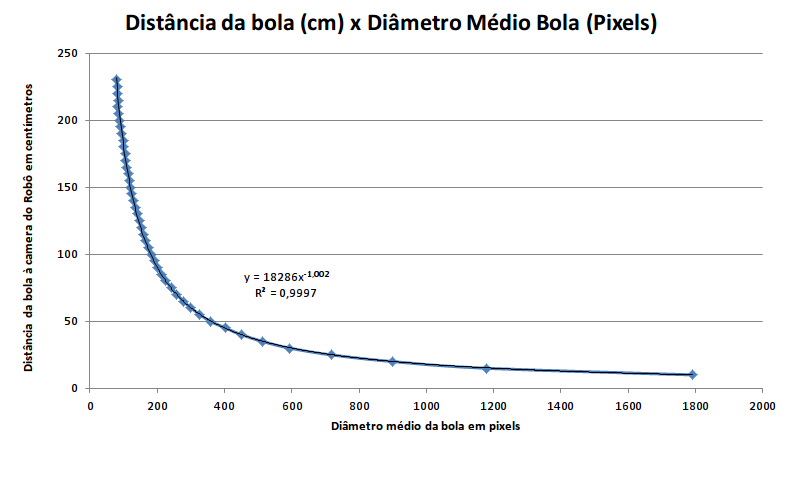
\includegraphics[width=15cm]{Imagens/Dist.png}
\DeclareGraphicsExtensions.
\caption*{Fonte: Autor.}
\label{Fig:DistBall}
\end{figure}

A função que relaciona o tamanho da bola em pixels com a distância da bola em centímetros foi extraída por meio de uma regressão não-linear exponencial, disponível no software Ms-Excel \cite{MS}, para a resolução de 1920x1080 pixels, bola de tamanho fixo e conhecido de 13 centímetros, onde \(D_{\text{Bola}}\) é a distância da bola ao robô em centímetros, e MRB é a média móvel do raio da bola em pixels.

O coeficiente de determinação \(R^2\) deve ser interpretado como a proporção de variação total da variável dependente do eixo Y (Distância da bola em centímetros) que é explicada pela variação da variável independente no eixo X (Tamanho da bola em pixels). Nesse caso pode-se concluir que 99,97 \% das variações de Y são explicadas pela variação de X. Como o gráfico foi plotado em relação ao diâmetro da bola , porém, como ambos os algoritimos fornecem como saída o raio da bola, se faz necessário a conversão do diâmetro em raio dividindo-o por dois.


\begin{equation} 
	%D_{bola} = 3,7.10^{-7} * MRB^4 -7.9e^{-5} * MRB^3 +6.2e^{-3} * MRB^2 -2.2e^{-1} * MRB + 3.7 
	%D_{bola} = 331.59-53.3*log(MRB-50);
	D_{bola} = \frac {\frac {18286} {2}} {MRB} \,\,\,\,\,\,\, \therefore \,\,\,\,\,\,\,\, D_{bola} = \frac {9143} {MRB}\,\,\,\,\,\, (cm)
\end{equation}

É claro que, haverá um erro de medição nessas fórmulas, já que foram calculadas sem oclusão e com o objeto inteiro no campo de visão da câmera, nesse caso, o erro será proporcional à oclusão.

\begin{comment}
\section{Determinação da distância do robô a outros robôs}

Para determinar as distâncias até os robôs adversários, ou até os companheiros de equipe é necessário que se possua todas as dimensões dos robôs da liga. Analisando os TDP's Artigos de descrição dos times de todos os robôs da liga KidSize, foram extraídos as alturas dos mesmos.
A tabela criada possui uma coluna referente ao número do time e uma ou mais colunas referente à altura do robôs de cada time, já que um time pode ter mais de um tipo de robô. 

Antes de se iniciar uma partida, o juiz procura os líderes de cada time para definição de suas respectivas cores. Duas cores são possíveis, o time vermelho tem uma coloração magenta e o time azul tem a cor ciano. Feita a escolha, os times devem revestir seus robôs com as cores definidas. A área mínima desses marcadores é 5x5 centímetros nos braços, pernas e tronco.

A detecção foi feita usando o descritor HAAR conforme parâmetros usados no capitulo ~\ref{HAAR-Boosting}

Somente dentro da janela de detecção do robô é feita uma segmentação da cor previamente escolhida no sistema HSV. Os valores foram discretizados em 20 valores para a matiz, 17 para a saturação e 17 para a intensidade.

Assim, se faz necessário encontrar uma fórmula que relacione a resolução da tela, o tamanho em pixels dos robôs e o tamanho real do robô com a sua distância. \citeonline{Bunden} utilizou uma fórmula que relaciona esses parâmetros para detecção da bola. 

Como o raio da bola e a largura do robô são unidimensionais seria possível utilizar a mesma fórmula, já que a relação .  

\begin{equation}
\label{Eq:Dis1}
d_{w} = \sqrt{ \frac {r_{cm}^2} { tan( \frac {\theta_{x}} {w_{img}} * r_{px}) }  - h_{cam}^2} 
\end{equation}

Onde \(d_{w}\) é a distância em centímetros da bola ao robô, \(r_{cm}\) é o raio real da bola em centímetros, \(\theta_{x}\) é o campo de visão horizontal da câmera em graus, \(w_{img}\) é a largura da imagem em pixels, \(r_{px}\) o raio da bola detectada em pixels e \(h_{cam}\) é a altura da câmera.

Como a janela de detecção é retangular o valor equivalente ao raio da bola foi substituído por metade da largura da janela de detecção \(J_{cm}\) e \(J_{px}\), como mostra a equação ~\ref{Eq:Dist2}.

\begin{equation}
\label{Eq:Dist2}
d_{w} = \sqrt{ \frac {      (\frac {J_{cm}}{2})^2    } { tan( \frac {\theta_{x}} {w_{img}} * \frac{ J_{px}} {2} ) }  - h_{cam}^2} 
\end{equation} 

Aqui, \(J_{cm}\) é a largura real do robô em centímetros extraída dos artigos de descrição dos times e \(J_{px}\) é a largura da janela de detecção em pixels, os outros parâmetros permanecem os mesmos da equação ~\ref{Eq:Dis1}

Duas limitações importantes devem ser observadas nessa abordagem, a primeira decorre da orientação do robô sendo observado, se ele estiver orientado à \(90^0\) com relação ao robô que está visualizando-o, sua largura em pixels será menor ou maior, dependendo do formato do robô e quão simétrico o mesmo é em relação ao plano sagital e/ou frontal, como mostra a figura ~\ref{Fig:Ori}, de forma que o cálculo de sua distância também será prejudicada. 

A função primordial da identificação dos robôs é, em primeira instância, iniciar em tempo hábil uma trajetória que evite uma colisão, em segunda instância e, talvez, mais complicada, envolve um procedimento de passes e jogadas ensaiadas entre robôs. Em ambos os casos uma variação de alguns centímetros no cálculo da distância não terá influência significativa, ao menos no estado atual da competição.

A segunda limitação aparece da própria equação utilizada e sua relação com o algoritmo de detecção. O algoritmo usado por \citeonline{Bunden} usa 3 recursos de checagem para a bola, inclusive um para oclusão, determinando com certa precisão os limites da bola. No caso da detecção dos robôs percebe-se que a detecção não tem limites tão bem definidos, de forma que uma abordagem prática utilizando dados reais dos próprios robôs poderiam apresentar melhores resultados em algum trabalho futuro. 


\pagebreak
\end{comment}
\section{Experimento - Detectando Robôs usando o Descritor HOG com o Classificador SVM}
\label{exp:HOG-SVM}

Sendo o algoritmo mais custoso computacionalmente, o reconhecimento de robôs roda com a resolução de 640x480 pixels e 15 quadros por segundo. O SVM foi treinado com um conjunto de imagens de pedestres humanos, os teste foram executados visando dois tipos de reconhecimento:
\begin{enumerate}
	\item SVM treinado com imagens humanas reconhecendo humanos- (Grupo de controle);
	\item SVM treinado com imagens humanas reconhecendo robôs;
	\item SVM treinado com imagens de robôs reconhecendo robôs.
\end{enumerate}


Para o descritor HOG um descritor padrão de 64x128 pixels foi usado da mesma forma que o artigo original, uma janela de 16x16 pixels, a célula que desliza pela imagem tem 32x32 pixels e um limiar de acerto de 0,5. Para o classificador SVM, o parâmetro de custo C ficou definido em 10 e o parâmetro $\Gamma$ ficou igual a 0.001, ambos escolhidos por uma busca em grade.

Como esperado, o classificador SVM, em conjunto com o descritor HOG, treinado com imagens de pessoas para reconhecimento de robôs é muito menos preciso do que o reconhecimento clássico de imagens de pessoas reconhecendo pessoas, entretanto, mesmo nessas circunstâncias, parece atingir a sua meta. Também foi reunida uma, mesmo que pequena, quantidade de imagens normalizadas contendo robôs, numa tentativa de verificar o quão bom esse algoritmo pode ser. Uma curva ROC foi plotada com as três situações, demonstrado na figura ~\ref{Fig:ROC} e o resultado de um quadro na figura ~\ref{Fig:Miltondet}:

\begin{figure}[!h!t!]
\centering \caption{Curvas ROC. A linha verde mostra o classificador clássico HOG-SVM, usado para reconhecimento de pessoas.
A linha vermelha demonstra o mesmo classificador treinado com pessoas usado para reconhecer robôs e a linha amarela mostra o classificador treinado com 100 imagens de robôs positivas e 100 imagens negativas usado na classificação dos robôs.}
\includegraphics[width=12cm]{Imagens/ROC1.png}
\DeclareGraphicsExtensions.
\caption*{Fonte: Autor \citefloat{Vilao}}
\label{Fig:ROC}
\end{figure}

As curvas ROC sugerem que o classificador treinado com imagens de robôs, mesmo com poucas imagens, parece ser, assintoticamente, melhor que a primeira abordagem usando o conjunto de imagens de pedestres. Nossa expectativa é fazer um classificador de robôs tão bom quanto o que reconhece pedestres. Devido a diversidade de robôs e sendo os seres humanos o nível máximo da forma humanoide, este classificador mostrou uma capacidade de generalização que poderia ser usada para reconhecer uma grande quantidade de robôs humanoides, dada uma quantidade suficiente de imagens de treinamento normalizadas.

\begin{figure}[!h!t!]
\centering \caption{Detecção do robô Milton usando imagens de pessoas como conjunto de treinamento.}
\includegraphics[width=7cm]{Imagens/Milton_Det.jpg}
\DeclareGraphicsExtensions.
\caption*{Fonte: Autor \citefloat{Vilao}}
\label{Fig:Miltondet}
\end{figure} 

É possível ver que a cabeça do robô não foi incluída no retângulo de detecção, talvez, pela falta de imagens normalizadas de boa qualidade ou, talvez, pelo fato da cabeça não estar em conformidade com a cabeça humana.
Como a aquisição de imagens tão específicas com uma mínima qualidade é de certa forma difícil de ser obter, a abordagem "Leave-One-Out" foi utilizada, já que lida bem com poucas amostras de treinamento.


\pagebreak

\section{Experimento - Detectando Robôs usando o Descritor HAAR com o Classificador Boosting}
\label{exp:HAAR-Boosting}
No contexto atual da liga KidSize da RoboCup, outros robôs não têm a necessidade de serem detectados enquanto estiverem a mais de 3 metros de distância, devido a sua velocidade de andar ser bastante reduzida, dessa forma, foi inserida uma limitação com relação à distância do robô a ser detectada.  Assim, a janela mínima de detecção foi definida com 150x150 pixels, ou seja, o menor objeto (robô) a ser detectado terá essa dimensão na imagem. O fato de limitar a janela de detecção mínima tem o principal objetivo de reduzir falsos positivos mas, também de acelerar o processo de detecção, já que menos janelas estarão contidas dentro da imagem. 

Durante o treinamento o número máximo de estágios foi determinado como sendo de 20 estágios, a taxa de acerto mínima foi configurada em 0.999, o parâmetro \(N_{\text{AmostrasPositivas}}\) após cálculo utilizando as equações ~\ref{eq1} e ~\ref{eq2} ficou fixada em 920 para 2135 imagens positivas e 1192 negativas, finalmente, a janela de amostragem foi de 150x150 pixels. O algoritmo foi implementado usando como classificador o k vizinhos mais próximos (K-nearest neighbors) com valor de k = 9. Valores como k=3, k =5 e k=7 foram escolhas claramente ruins, já que geraram diversos falsos positivos. O valor de k=11 teve bons resultados mas, também ignoraram o objeto em diversas circunstâncias. Maiores valores de k não geraram classificação. Mesmo apresentando falsos positivos o Haar conseguiu identificar o robô em diversas situações. Na figura ~\ref{fig:Art} uma sequência de quadros do robô B2 sendo identificado, com o uso do Haar, em um campo de futebol com grama sintética. 

\begin{figure}[!h!t!]
    \centering \caption{Rastreamento do robô B2 usando características HAAR no campo de futebol com grama artificial.}
    \subfloat[]{{\includegraphics[width=4.5cm]{Imagens/Darwin01.png} }}
    \qquad
    \subfloat[]{{\includegraphics[width=4.5cm]{Imagens/Darwin02.png} }}
    \qquad
    \subfloat[]{{\includegraphics[width=4.5cm]{Imagens/Darwin03.png} }}
    \qquad
    \subfloat[]{{\includegraphics[width=4.5cm]{Imagens/Darwin04.png} }}
    \qquad
    \subfloat[]{{\includegraphics[width=4.5cm]{Imagens/Darwin05.png} }}
    \qquad
    \subfloat[]{{\includegraphics[width=4.5cm]{Imagens/Darwin06.png} }}
    \qquad
    \subfloat[]{{\includegraphics[width=4.5cm]{Imagens/Darwin07.png} }}
    \qquad
    \subfloat[]{{\includegraphics[width=4.5cm]{Imagens/Darwin08.png} }}
    \qquad
    \subfloat[]{{\includegraphics[width=4.5cm]{Imagens/Darwin09.png} }}
    \qquad
    \subfloat[]{{\includegraphics[width=4.5cm]{Imagens/Darwin10.png} }}
    \qquad
    \subfloat[]{{\includegraphics[width=4.5cm]{Imagens/Darwin11.png} }}
    \qquad
    \subfloat[]{{\includegraphics[width=4.5cm]{Imagens/Darwin12.png} }}
    \caption*{Fonte: Autor}
    \label{fig:Art}
\end{figure}



\section{Discussão - Comparando os dois descritores e seus classificadores} 
\label{exp:comp}

Diferentemente do experimento apresentado na seção ~\ref{exp:HOG-SVM} nessa seção, as imagens utilizadas para treinamento das técnicas HOG-SVM e HAAR-Adaboost foram as mesmas, ou seja, 2135 imagens positivas e 1192 imagens negativas. Os parâmetros se mativeram os mesmos dos experimentos das seções ~\ref{exp:HOG-SVM} e ~\ref{exp:HAAR-Boosting}.
Duas curvas ROC foram plotadas e os resultados estão na figura ~\ref{fig_rocHH}. A quantidade de quadros por segundo foi extraída usando um código simples que armazenava e contava os quadros dentro do período de 5 minutos, sendo portanto o resultado apresentado na figura ~\ref{fig_fps} a média de quadros por segundo em 5 minutos. Esse período foi escolhido devido a limitação de tempo dos videos que foram usados para o teste. Na figura ~\ref{fig_He}, os resultados dos dois métodos aplicados à mesma imagem do robô Bold Hearts. É possível verificar que não há grande diferença entre as duas detecções.
O descritor HAAR teve um desempenho melhor que o descritor HOG em termos de velocidade, especialmente nas maiores resoluções. Entretanto quando o robô foi levado para o ambiente real, a iluminação se tornou um verdadeiro problema. Para ambos os algoritmos foi necessário incluir imagens negativas referentes ao ambiente. Na figura ~\ref{fig_rocHH} uma curva ROC que compara as capacidades e limitações dos dois algoritmos. 

\begin{figure}[!h!t]%
    \centering  \caption{Identificação do Robô Bold Hearts \cite{Bold} da universidade de Hertfordshire usando HOG-SVM (Figura a) e HAAR-Adaboost (Figura b).}%
    \subfloat[HOG - SVM]{{\includegraphics[width=10cm]{Imagens/HeartsHOG.png} }}%3.65
    \qquad
    \subfloat[HAAR - Boosting]{{\includegraphics[width=10cm]{Imagens/HeartsHAAR.png} }}%
\caption*{Fonte: Quadro extraído do vídeo de qualificação do time Bold Hearts \cite{Bold} disponível em \citefloat{BoldHearts}.}
    \label{fig_He}%
\end{figure}

\begin{figure}[!h!t!]
\centering \caption{Curvas ROC. A linha verde mostra o algoritmo HOG-SVM clássico treinado com imagens de robôs usado para detecção de robôs.
A linha vermelha demonstra o resultado do classificador HAAR-AdaBoost treinado com o mesmo propósito.}
\includegraphics[width=12cm]{Imagens/ROCHH.png}\\
\DeclareGraphicsExtensions.
\caption*{Fonte: Autor.}
\label{fig_rocHH}
\end{figure}

As duas curvas ROC apresentadas na figura ~\ref{fig_rocHH} sugerem que os classificadores treinados parecem ser equivalentes. Devido à diversidade de robôs ambos os classificadores demonstraram capacidade de generalização que pode reconhecer diversos tipos de robôs dadas imagens de treinamento normalizadas suficientes.

Outro parâmetro de desempenho utilizado foi o de resposta dos algoritmos em quadros por segundo. É vital para um robô jogador de futebol que consiga detectar outros robôs em tempo real. A comparação desses parâmetros de desempenho estão na figura ~\ref{fig_fps}, esta informação é particularmente vital quando se trata de um robô que precisa agir rapidamente.

\begin{figure}[!h!t!]
\centering \caption{Desempenho dos descritores HAAR-AdaBoost e HOG-SVM em termos de quadros por segundo após processamento.}
\includegraphics[width=12cm]{Imagens/FPS.png}
\DeclareGraphicsExtensions.
\caption*{Fonte: Autor}
\label{fig_fps}
\end{figure}

Os resultados mostram alguma vantagem para o HAAR-Adaboost em quadros por segundo, que pôde ser utilizado em full-hd 1920x1080 pixels mas, com alguns falso positivos, já que é uma técnica sensível à mudanças de iluminação. Já o HOG-SVM foi mais preciso em termos de detecção, porém com a limitação da taxa de velocidade e por consequência a resolução máxima de 640x480 pixels. Nas figuras ~\ref{fig:Mix1} e ~\ref{fig:Mix2} as mesmas imagens demonstrando as detecções para os dois algoritmos. Nessas figuras as detecções mostraram alguma vantagem para o HOG, que demonstrou mais estabilidade detectando menos falso positivos.

Aqui cabe uma ressalva, quando se trata de avaliar os descritores, os parâmetros escolhidos e o hardware foram verdadeiramente responsáveis pelo desempenho geral dos dois algoritmos.

O tempo gasto no treinamento e na normalização e redimensionamento das imagens também foi uma questão complicada. Enquanto o HOG-SVM determinava todas as características por si só e levava no máximo 2 horas para efetuar o treinamento, o HAAR-Adaboost precisava que uma pessoa determinasse onde os objetos estavam em cada imagem positiva e seu treinamento levou de 5 a 12 horas para ser concluído. É válido lembrar que as imagens positivas do HOG-SVM precisaram ser redimensionadas o que levou um tempo considerável.


\begin{figure}[!h!t!]%
    \centering  \caption{Vários robôs identificados usando o HOG-SVM e o HAAR-AdaBoost.}%
    \subfloat[HOG - SVM]{{\includegraphics[width=15cm]{Imagens/MixHOG.png} }}%3.65
    \qquad
    \subfloat[HAAR - Boosting]{{\includegraphics[width=15cm]{Imagens/MixHAAR.png} }}%
\caption*{Fonte: Quadro extraído do vídeo de qualificação do time Bold Hearts \cite{Bold} disponível em \citefloat{BoldHearts}.}
    \label{fig:Mix1}%
\end{figure}

\begin{figure}[!h!t!]%
    \centering  \caption{Quadro de captura do robô B2 identificando vários robôs usando o HOG-SVM (Figura a) e o HAAR-AdaBoost (Figura b).}%
    \subfloat[HOG - SVM]{{\includegraphics[width=15cm]{Imagens/CIT01HOG.png} }}%3.65
    \qquad
    \subfloat[HAAR - Boosting]{{\includegraphics[width=15cm]{Imagens/CIT01HAAR.png} }}%
\caption*{Fonte: Autor.}
    \label{fig:Mix2}%
\end{figure}

\pagebreak





%%===============================================================================



%*********************************************************************************************************************************************
%---------------------------------------------------------------------------------------------------------------------------------------------
%-------------------------------------  CAPÍTULO 6 - CONCLUSÃO -------------------------------------------------------------------------------
%---------------------------------------------------------------------------------------------------------------------------------------------
%*********************************************************************************************************************************************

\chapter{Conclusão}

Esse trabalho apresentou uma solução de visão computacional para o ambiente KidSize, robusto à mudanças de iluminação, usando algoritmos de visão básicos e bem conhecidos, entretanto, o ambiente real provou ser bastante desafiador.

Houveram diversas mudanças nas regras da RoboCup para a categoria entre os anos de 2014 e 2015, as duas principais mudanças são relativas às cores do gol(amarelo) e da bola (laranja), que passaram a ter suas cores alteradas para a cor branca. 

Essas mudanças, apesar de drásticas para o domínio proposto, parecem levar ao encontro da meta da RoboCup. A abordagem apresentada permitiu que diversas técnicas pudessem ser utilizadas para identificar características como cores, texturas, bordas e contornos.

Dada a limitação da aplicação em tempo real, HAAR teve um melhor desempenho levando-se em consideração apenas a velocidade de computação. No entanto, possui alguns problemas com iluminação e, portanto, têm uma alta taxa de falsos alarmes especialmente em ambientes reais e complexos. Os resultados mostram algumas vantagens para a técnica de Haar em quadros por segundo, de forma que pode ser executado em Full HD, mas com alguns falsos positivos, uma vez que é uma técnica muito sensível às mudanças de iluminação e, embora o descritor HOG demonstrou mais precisão em termos de detecção, mostrou ter uma limitação da taxa de velocidade e resolução máxima de 640x480 pixels. Quando se trata de avaliar os descritores e seus classificadores a escolha dos parâmetros e o hardware utilizado tiveram fortes influências no desempenho total do sistema.

O tempo gasto em treinamento também foi uma questão complicada. Enquanto Hog determinava todas as características por si só e levava apenas alguns minutos para o treinamento, o HAAR precisava de uma pessoa para determinar onde os objetos se encontravam na imagens, e levando de 5 à 10 horas para ser concluído. As imagens de treinamento usadas para classificação usando o descritor HOG tiveram que ser reduzidas e normalizadas para o tamanho proposto no trabalho original de \citeonline{Dallal}.

Na competição, no entanto, fazer o robô ignorar o ambiente de fundo provou ser uma tarefa muito desafiadora. Dessa forma, dado o hardware utilizado e os objetivos propostos, o descritor HAAR parece ser mais a técnica mais apropriada para o domínio proposto, principalmente por sua  velocidade de processamento. 

Construir uma base de imagens de robôs, a variedade de robôs atuantes na liga é muito grande e para se ter um classificador confiável, é necessário um conjunto de imagens de treinamento provenientes dos mais diversos tipos de robôs, assim como, suas respectivas dimensões.

O time qualificou-se e participou da RoboCup, liga KidSize, pela primeira vez em 2014, atingindo a segunda fase de grupos, terminando entre os 16 melhores colocados de 23 inscritos. 



\section{Contribuições}

As seguintes contribuições são decorrentes desse, e são citadas:

\begin{itemize}
	\item a construção do sistema de visão computacional do robô para a competição do time RoboFEI em diversos campeonatos de futebol \cite{Vilao} \cite{perico2014hardware};
	%\item disponibilização do banco de imagens normalizadas de robôs e bolas utilizadas no treinamento do HAAR e do HOG;
	\item quebra de um paradigma para o domínio, onde se acreditava que era necessário o uso de segmentação por cores, com o desenvolvimento de um sistema de visão computacional para identificação da bola que não é dependente de segmentação de cores;
	\item um sistema de detecção de robôs ainda pouco explorado nesse domínio \cite{Vilao2};
	\item a equipe foi campeã Latino-Americano de futebol de robôs \cite{LARC2014} e ficou entre os 16 melhores colocados na categoria KidSize da Robocup nos anos de 2014 em João Pessoa \cite{JP2014} e 2015 na cidade de Hefei na China \cite{JP2015}.
\end{itemize}


\section{Trabalhos Futuros}

Certos aspectos do desenvolvimento do sistema de visão computacional foram abordados no presente visando solucionar os mais diversos problemas inerentes desse tipo de sistema. Com o intuito de melhorar, expandir ou modificar o presente serão citados alguns itens que surgiram durante a elaboração do presente e que são descritos brevemente como possíveis trabalhos futuros.


\begin{enumerate}
\item uma comparação entre o HOG e o HAAR foi proposta, porém outras técnicas podem ser utilizadas, como por exemplo, o CenTrist. Trata-se de uma técnica computacionalmente eficiente para capturar e determinar contornos comparado com o HOG, mas ainda há a escassez de artigos que implementaram e testaram a precisão do descritor Centrist para identificar robôs;

\item um estudo para identificar os níveis de processamento e robustez de redes neurais profundas (Deep Neural Networks - DNN) para identificação de robôs e outros objetos com o video de uma câmera em movimento também pode ser vislumbrado;

\item implementar o filtro de Kalmman no rastreamento da bola pode ser uma alternativa para o filtro de partículas;

\item limitar a área de rastreamento da bola, já que a bola precisa estar no campo, é possível considerar que a bola estará contida em uma região predominantemente verde;

\item uma comparação entre o Haar e a transformada de Hough para círculos para a bola laranja;

\end{enumerate}

%%===============================================================================



\bibliography{Bibliografia}

%\appendix
%\chapter{Algoritmo de Detecção da Bola Laranja} 
\label{chap:apendiceBolaLaranja}
\section{Algoritmo de rastreamento da bola - Círculos de Hough.}

\begin{algorithm}

\Entrada{Abre Captura da Câmera (Dispositivo 0)}
\Se{Captura vazia}
	{Erro! Dispositivo não está pronto.
	Aborte Algoritmo.
		}

\Enqto{ Não for pressionada a tecla esc e Quadro não vazio}
{

Extraia um quadro RGB da captura, converta para uma imagem HSV.

\begin{equation}
     \centering
    	H = \left\{
		\begin{array}
		{ccl} 
		$$\theta, 	& Se B  \leq  G $$\\
		$$360 - \theta,	& Se B  >  G $$
		\end{array} 
\right.
\end{equation}

\begin{equation}
	\theta  =  \cos^-{^1} \left[  {   \frac {  \frac {1} {2} * [(R -G) + (R-B)]}  {  \sqrt{[(R -G)^2 + (R -B)(G -B)]}   }    }\right]
\end{equation}

\begin{equation}
	S  =  1 - { \frac {3} {(R+G+B)} } * [min (R,G,B)]
\end{equation}

\begin{equation}
	I  =  { \frac {1} {3}} * {(R+G+B)}
\end{equation}



\Entrada{Tabela de pesquisa (LUT). (0<H<35, 0<S<180, 0<V<255)}

\ParaTodo {Pixel dentro da imagem HSV e dentro dos limites da LUT}
	{Altere o valor do Pixel de uma matriz binária na mesma posição}

Na matriz binária aplique Erosão seguida da Dilatação. ( 5x5 Pixels)

Aplique filtro espacial. (Gaussiana 9x9 Pixels)

Transformada de Hough para círculos:

- Atualize a média móvel do raio (MRB) e da posição XY dos círculos encontrados.

\begin{equation} 
	D_{bola} = \frac {9143} {MRB}
\end{equation}\\

Armazene \(D_{bola}\), a posição dos servos Pan-Tilt em graus e da bola em pixels.
}

\Retorna \(D_{bola}\)

\caption[Algoritmo de rastreamento da bola - Círculos de Hough.]{Fonte: Autor.}
\label{lst:algBall}
\end{algorithm}


\chapter{Algoritmo para divisão do Quadro} \label{chap:apendiceDivQuadro}

\section{Algoritmo para buscar e centralizar o objeto.}
\begin{algorithm}

Divida o quadro de captura em 3 regiões horizontais, sendo a região central com 5\% da resolução horizontal.\\
Divida o quadro de captura em 3 regiões verticais, sendo a região central com 5\% da resolução vertical.\\
\Enqto{Quadro não vazio}
{
	\Se{Dentro do quadro houver objeto}
		{
		Encontre em qual região o objeto se encontra usando sua posição.\\
				\Se {O objeto estiver na região 5 (central)} 
					{Mantenha o objeto nessa região parando o movimento}
				\Se {O objeto estiver nas regiões 1, 4 e 7} 
					{Some a posição atual do servo com a quantidade de graus para o pan}
				\Se {O objeto estiver nas regiões 3, 6 e 9} 
					{Subtraia a posição atual do servo com a quantidade de graus para o pan}
				\Se {O objeto estiver nas regiões 1, 2 e 3} 
					{Some a posição atual do servo com a quantidade de graus para o tilt}
				\Se {O objeto estiver nas regiões 7, 8 e 9} 
					{Subtraia a posição atual do servo com a quantidade de graus para o tilt}
		Guarde posição dos servos\\
		}
		\Senao
		{		
		Chame algoritmo de busca \ varredura
		}
	
}
\Retorna \(Posicao do Servo\)

\caption[Algoritmo para buscar e centralizar o objeto]{Fonte: Autor}
\label{lst:algCent}
\end{algorithm}



\chapter{Algoritmo para Identificação de Robôs. (HOG-SVM)} \label{chap:apendiceHOG}

\section{HOG-SVM Offline}
\begin{algorithm}


\Entrada{Conjunto de imagens positivas - Contém robôs participantes}
\Entrada{Conjunto de imagens negativas - Não contém robôs}

Extraia, do diretório de imagens negativas, todas as imagens que possuam tamanho e extensão compatíveis (jpg,jpeg,png,bmp)

Calcule o histograma de gradientes para todas as imagens.

Armazene o vetor de características (descritores) de cada uma das imagens negativas.

Extraia, do diretório de imagens positivas, todas as imagens que possuam tamanho e extensão compatíveis (jpg,jpeg,png,bmp)

Calcule o histograma de gradientes para todas as imagens desse diretório.

Armazene o vetor de características (descritores) de cada uma das imagens positivas.

Armazene o vetor de características (descritores) de cada uma das imagens negativas.

\Entrada{Vetores de características (descritores) das imagens positivas}
\Entrada{Vetores de características (descritores) das imagens negativas}

Determine os vetores de suporte e o hiperplano que melhor separa as duas classes usando o SVM.

\Entrada{Tabela com todas as alturas de todos os robôs de todos os times}
\Entrada{Tabela com a cor do time adversário}

\label{lst:algROF}
\caption[Algoritmo para Identificação de Robôs. (HOG-SVM Offline)]{Fonte: Autor.}
\end{algorithm}

\pagebreak

\section{HOG-SVM Online}

\begin{algorithm}


\Entrada{Hiperplano proveniente do SVM}
\Entrada{Aquisição da câmera}

\Enqto{ Quadro não vazio}
{
Calcule o histograma de gradientes da imagem adquirida da câmera

Extraia o vetor de caracterísiticas (descritores) da imagem adquirida.

Use o SVM para classificar o vetor de caracterísiticas da imagem adquirida.

	\Se {Houver robô presente na imagem}
	{
		Para cada bloco da imagem adquirida, encontre em qual bloco do histograma normalizado o robô se encontra\\

		Calcule sua altura em pixels\\

		Armazene o centro do bloco e a altura em pixels\\

		Segmentação da cor do time.\\

		Se a área na qual o robô for identificado conter o centroide referente à cor do time\\

		Busque na tabela de alturas qual a altura em centímetros do robô que foi identificado\\

		Calcule sua distância real até o robô em centímetros\\
	}

}
\caption[Algoritmo para Identificação de Robôs. (HOG-SVM Online)]{Fonte: Autor.}
\label{lst:algROn}
\end{algorithm}


\chapter{Algoritmo para Identificação de Robôs. (HAAR-Adaboost)} \label{chap:apendiceHAAR}

\section{HAAR-Adaboost Offline}
\begin{algorithm}

\Entrada{Conjunto de imagens positivas - Contém robôs participantes}
\Entrada{Conjunto de imagens negativas - Não contém robôs}

\Entrada{Posição dos robôs contidos nas imagens positivas}

\ParaTodo {Estágio da árvore e para todas as imagens}
{
\Enqto{\(Min_{\text{TaxaAcerto}}\) = 0,999 não atingida}
	{
	Extraia as características de HAAR para as imagens positivas.\\
	Execute o Adaboost conforme algoritmo ~\ref{lst:algHaar} usando como parâmetros:\\
		- Tamanho da amostra = 20x20 Pixels;\\
		- Tamanho mínimo do objeto = 30x30 Pixels;\\
		- Tamanho máximo do objeto = Resolução vertical x \( \frac {Resolução Horizontal}{2}\) Pixels\\
		- Classificador 8 Vizinhos mais próximos. \\
	}
	Armazene a hipótese final do estágio.\\
}
	Armazene a hipótese final em um arquivo .xml

\caption[Algoritmo de Identificação de robôs. (HAAR-Adaboost Offline)]{Fonte: Autor ``Adaptado de'' \citefloat{Adaboost} }
\label{lst:algHaarOF}
\end{algorithm}

\pagebreak

\section{HAAR-Adaboost Online}
\begin{algorithm}

\Entrada{Árvore proveniente do Adaboost (Arquivo .xml)}

\Entrada{Aquisição da câmera}

\Enqto{ Quadro não vazio}
{

Extraia o vetor de caracterísiticas (descritores) da imagem adquirida.\\
Percorra os nós (Estágios) da árvore presentes no arquivo xml encontrando a melhor classificação para a imagem adquirida\\

	\Se {Houver robô presente na imagem}
	{
		Para cada bloco da imagem adquirida, encontre em qual bloco o robô se encontra\\

		Calcule sua altura em pixels\\

		Armazene o centro do bloco e a altura em pixels\\

		Segmentação da cor do time.\\

		Se a área na qual o robô for identificado conter o centroide referente à cor do time\\

		Busque na tabela de alturas qual a altura em centímetros do robô que foi identificado\\

		Calcule sua distância real até o robô em centímetros\\
	}
}

\caption[Algoritmo de Identificação de robôs. (HAAR-Adaboost Online)]{Fonte: Autor ``Adaptado de''\citefloat{Adaboost} }
\label{lst:algHaarOn}
\end{algorithm}


	


\anexos

\chapter{Média Móvel}
\label{Anexo:MM}
 \section{Séries Temporais}


O conceito de séries temporais está relacionado a um conjunto de observações de uma determinada variável feita em períodos sucessivos de tempo e ao longo de um determinado intervalo. Podemos citar como exemplos as cotações diárias da taxa do dólar, as vendas mensais de um determinado produto, a taxa de desemprego de um país, e etc. Segundo \citeonline{Morettin} os objetivos de se analisar uma série temporal são os seguintes: 

\begin{enumerate}
\item Descrição: propriedades da série como, por exemplo, o padrão de tendência, a existência de alterações estruturais, etc. 
\item Explicação: construir modelos que permitam explicar o comportamento da série no período observado. 
\item Controle de Processos: por exemplo, controle estatístico de qualidade. 
\item Previsão: prever valores futuros com base em valores passados. 
\end{enumerate}

Existem inúmeros métodos para se fazer previsão de séries temporais, desde os mais complexos que envolvem diferentes parâmetros aos métodos mais simples e de fácil entendimento. Para \citeonline{Makridakis} o fato de se utilizar métodos estatísticos mais complexos não significa necessariamente uma melhora nos resultados da previsão. Métodos simples podem apresentar resultados satisfatórios sobre certas condições, além de permitir uma total compreensão de suas limitações facilitando assim a interpretação dos resultados. Sendo assim deve-se primeiro avaliar os benefícios de se utilizar um método simples ou um mais complexo antes de se iniciar a previsão em uma determinada aplicação.

\section{Métodos Simples de Previsão de Série Temporal}

Muitos estudos envolvendo séries temporais têm como objetivo fazer previsões. Existem alguns métodos de previsão simples e que efetuam a previsão de valores futuros da série temporal através das observações de valores passados da série em interesse. Segundo \citeonline{Morettin} o propósito destes métodos é identificar um padrão básico presente nos dados históricos da série e através deste padrão prever valores futuros.
Estes métodos simples têm uma grande popularidade, pois são simples de programar, e o custo computacional é muito pequeno além de obter uma razoável previsão. Dentre estes métodos podemos citar a média móvel, o alisamento exponencial simples e linear e também o alisamento exponencial sazonal e linear de Winter.

Os modelos de média móvel utilizam como previsão para um determinado período no futuro a média das observações passadas. As médias móveis podem ser simples, centradas ou ponderadas. Para os modelos de média móvel simples que são os modelos utilizados neste trabalho podemos definir sua equação como:  

\begin{equation} 
	x_{t} = \frac {[x_{t-1} + x_{t-2} + x_{t-2} + . . . + x_{t-n}]}  {n}
\end{equation}

Na equação acima n representa o número de observações incluídas na média Xt, ou seja, n (também pode ser chamado de janela de observações) pode ser considerado como um parâmetro a ser ajustado. Neste caso quanto maior for a janela de observações maior o efeito de alisamento na previsão. Sendo assim, se a série em estudo apresentar muita aleatoriedade ou pequenas mudanças em seus padrões um número maior de observações podem ser utilizadas no cálculo da média móvel, ou seja, podemos dizer que a média móvel neste caso fica mais imune a ruídos e movimentos curtos. Já para o caso de séries que apresentam pouca flutuação aleatória nos dados ou mudança significativa, um número menor deve ser usado para o tamanho da janela de observações, pois caso contrário a série prevista poderá reagir de maneira muito lenta as estas mudanças significativas.   Para \citeonline{Morettin} o termo média móvel é utilizado porque à medida que a próxima observação está disponível, a média das observações é recalculada, incluindo esta observação no conjunto de observações e desprezando a observação mais antiga, conforme podemos visualizar na figura ~\ref{Fig:MMA}:

\begin{figure}[!t]
\centering
\includegraphics[width=5.5in]{Imagens/MM.png}
\DeclareGraphicsExtensions.
\caption{Cálculo das Médias Móveis Simples.}
\label{Fig:MMA}
\end{figure}

Na figura acima o valor N corresponde ao número de observações (tamanho da janela igual a três) a ser utilizado para o cálculo da média móvel simples. Podemos perceber claramente que para cada nova janela de três dias a ser formada, a observação mais antiga é desprezada, e uma nova observação é inserida no conjunto N para o próximo cálculo. 


\end{document}
